\documentclass[manuscript,screen,review]{acmart}

%% ===================== 中文支持 =====================
%% 本文为中文稿,必须用 XeLaTeX 编译(pdfLaTeX 无法处理中文)。
%% scheme=plain 让 ctex 只接管中文字体与断行,不改写 acmart 的标题版式与章节名,
%% 否则两者会争夺 \section 的定义而报错。
%% fontset=windows 使用系统的宋体/黑体;若改到 Linux 或 Overleaf 上编译,
%% 把它换成 fontset=fandol(TeX Live 自带,无需系统字体)。
\usepackage[UTF8,scheme=plain,fontset=windows]{ctex}

\usepackage{algorithm}
% Use algorithmicx + algpseudocode: provides \Require, \Ensure, \State, and \Comment
\usepackage{algorithmicx}
\usepackage{algpseudocode}
\usepackage{tikz}
% Load common tikz libraries used in figures (positioning provides the "of" syntax)
\usetikzlibrary{positioning,arrows.meta,calc,shapes,shadows}
% color support for \textcolor used inside algorithms
\usepackage{xcolor}
% Math packages required for \text and bold symbols inside math
\usepackage{amsmath}
\usepackage{bm}
\usepackage{multirow}
% Enable list customization (leftmargin, itemsep, etc.) used in the document
\usepackage{enumitem}
% Ensure header height is sufficient for fancyhdr
\setlength{\headheight}{20.48303pt}
% Visible placeholder for numbers still awaiting the controlled matrix run.
% Every occurrence must be gone before submission: grep for \TBD.
\newcommand{\TBD}[1]{\textcolor{red}{\textbf{[TBD:} #1\textbf{]}}}
% theorem environments used in the document
\usepackage{amsthm}
\newtheorem{assumption}{假设}
\newtheorem{problem}{问题}
% Define remark environment (was missing and caused compilation errors)
\newtheorem{remark}{注}
% acmart 自己已经定义了 proposition 与 lemma(英文名),不能用 \newtheorem 重名覆盖,
% 也没有提供改名接口,故另起两个中文环境,正文用 prop / lem。
\newtheorem{prop}{命题}
\newtheorem{lem}{引理}

%% 浮动体与交叉引用的中文名称。ctex 用 scheme=plain 载入时不会改这些,须手工设定。
\renewcommand{\figurename}{图}
\renewcommand{\tablename}{表}
\floatname{algorithm}{算法}
\renewcommand{\proofname}{证明}

%% ===================== 全文图表的重建顺序 =====================
%% 有先后依赖,按序执行。前两步在 clbs/ 目录下跑,后两步在仓库根目录跑。
%%
%%  1. 主结果(约 6 小时,决定下面所有数字):
%%       py -u -m tools.baseline_ladder --budget 90 \
%%          --seeds 42,7,2024,13,1,99,123,777,31415,8      -> output/baseline_ladder.csv
%%  2. 三个配套批次(可在 1 之后依次跑,彼此无依赖):
%%       py -u -m tools.prune_ablation --budget 90         -> output/prune_ablation.csv
%%       py -u -m tools.ladder_diag  --budget 90           -> output/ladder_cost.csv
%%                                                            output/ladder_convergence.csv
%%                                                            output/case_study/*.json
%%     注意:三者与第 1 步都用挂钟预算,故**不可并行**——并行会互相偷走评价次数,
%%     恰好破坏本文第 5.1 小节所主张的同挂钟协议。这一条不是洁癖,是结果的前提。
%%  3. 表与宏(秒级):
%%       py paper01/tab/gen_tables_ladder.py
%%     它写出 tab/*.tex,并把下面这整块宏定义打印出来供替换;两者同源,故不会互相矛盾。
%%  4. 图(秒级,需要 matplotlib):
%%       py paper01/fig/render_all.py         (按数据可用性逐张渲染,缺数据的跳过)
%%     单张重绘:英文脚本与对应 *_CN.py 成对;正文引用中文版 PDF。
%%       fig_framework_CN.py、fig_motivating_CN.py、fig_prediction3_CN.py、
%%       fig_convergence_CN.py、fig_protocol_CN.py、fig_protocols_CN.py、
%%       fig_theta_CN.py、fig_case_gantt_CN.py、fig_case_chain_CN.py
%%     加环境变量 CLBS_FIG_PNG=1 可同时出 png 便于预览。
%%  5. 自检(秒级,无需 TeX 引擎):
%%       py paper01/check_tex.py
%%     它检查未定义宏、写死的数字、括号与环境配对、悬空的交叉引用,以及残留待办。
%%
%% 数据完备性(2026-08-16 复核):九张图的数据均已落盘,无待补项。
%% 此处原有一条"fig_theta.pdf 的定价扫描数据未落盘"的备注,系误记——
%% clbs/experiments/theta_sweep.csv 与 theta_sweep_gen.csv 两个 CSV 均在盘上,
%% 图注处已作同样更正,现删除该备注以免两处再度矛盾。

%% ===================== 主结果数字的单一来源 =====================
%% 论文正文一律引用下面的宏,不要在别处写死百分数。上一版论文的教训是同一个数字
%% 散落在摘要、引言、贡献列表和实验章里,换一批数据就得逐处找,漏一处就自相矛盾。
%%
%% 数据来源:clbs/output/baseline_ladder.csv,由 clbs/tools/baseline_ladder.py 生成;
%% 复现命令(在 clbs/ 目录下):py -u -m tools.baseline_ladder --budget 90 --seeds ...
%% 口径:10 个受控算例 x 10 种子 = 100 配对,同挂钟预算,配对 Wilcoxon 符号秩检验。
%%
%% 数值取自 10 算例 x 10 种子 = 100 配对(output/baseline_ladder.csv, 2026-08-08 落盘)。
%% 由 tab/gen_tables_ladder.py 从同一 CSV 复算;表与正文同源。
%%
%% !! 相对 4 种子初跑,有三条叙事必须跟着改写,不能只换数字:
%% !!  (1) 开环下试探派车现已显著(4.59%, p<1e-4),不再是"几乎不值钱";
%% !!  (2) 端到端 21.35% < 独立乘积 22.6%,正交互论断不成立,改为近加性/略亚加性;
%% !!  (3) B NA/NM 0.5 的 B0->B1 已翻为负(闭环仍有益),而 B 族大车队两格上
%% !!      B1->B2 为正。**注意**:这一条一度被写成"适用上界",2026-08-16 复核逐格
%% !!      显著性后已撤回,原因见下面车机比族那一段的说明,不要照抄本行。
%%
%% 逐格表(tab_bytag)与本块用**同一个**估计量:逐对相对增益在种子上的均值。
%% 上一版逐格用的是"两档均值之比",于是把十格一平均得到 -20.0%/-2.9%,与这里的
%% -18.86%/-2.45% 对不上,读者手算即可发现。设计是平衡的(每格 10 种子),改成同一
%% 估计量之后十格均值精确等于本块的合计值。代价是逐格表的增益列不再能由同一行的
%% 两个均值列反推,该口径已写进表注。
\newcommand{\NCases}{10}
\newcommand{\NSeeds}{10}
\newcommand{\NPairs}{100}
% 闭环本身的价值(固定派车方式,只动"拥堵是否进入搜索目标")
\newcommand{\GainLoopRule}{18.86\%}      % B0  -> B1 ,规则派车下
%% p 值一律是**Holm 校正后**的值,族 = 表 tab:main 的五个对比。校正对这五个对比是
%% 惰性的(逐个与校正前相同),因为最大的那个 p 恰是最大者、乘数为 1,其余小到乘 5
%% 仍远小于阈值。这一点本身要能从正文说出来,故此处标明口径而不是留给读者猜。
%%
%% !! 约定:所有 P 开头的宏\emph{自带关系符}("<" 或 "="),故正文一律写 $p\PLoopRule$,
%% !! 前面**不要**再加等号。理由是 Wilcoxon 在 <1e-4 时回报 0.0000,而把它印成
%% !! "p=0.0000" 等于宣称 p 为零;关系符若留在正文,重跑一次把某个 p 压到阈值以下,
%% !! 该处就会渲染成 "p=<10^{-4}" 而无人察觉。gen_tables_ladder.py 的 pmac() 负责
%% !! 按数值挑选关系符,故这条约定是由生成器强制的,不靠记忆。
\newcommand{\PLoopRule}{<10^{-4}}
\newcommand{\GainLoopProbe}{17.75\%}     % B0+ -> B2 ,试探派车下
\newcommand{\PLoopProbe}{<10^{-4}}
% 预约表感知派遣的价值(固定闭环与否,只动派车决策)
\newcommand{\GainProbeOpen}{4.59\%}      % B0  -> B0+,开环下,现已显著
\newcommand{\PProbeOpen}{<10^{-4}}
\newcommand{\GainProbeLoop}{2.45\%}      % B1  -> B2 ,闭环内(被大车队两格拖低)
\newcommand{\PProbeLoop}{=0.0054}
% 端到端:文献结构 -> 本文
\newcommand{\GainEndToEnd}{21.35\%}      % B0  -> B2
\newcommand{\PEndToEnd}{<10^{-4}}
\newcommand{\WinEndToEnd}{94}
\newcommand{\LoseEndToEnd}{5}
%% ---- 效应量:Hodges--Lehmann 伪中位数与 95% 分布无关置信区间 ----
%% 上面那些 Gain 宏是"逐对相对增益在配对上的均值",它没有精度陈述,且与旁边的
%% Wilcoxon p 值不同源(后者用秩)。HL 伪中位数正是符号秩检验对应的点估计,其区间
%% 由同一个零分布读出,故点估计 / 区间 / p 值三者同源。区间由 clbs/algorithm/stats.py
%% 的 hodges_lehmann_ci 按 Hollander--Wolfe 口径给出($n=100$ 走正态近似)。
%% 两个宏都取绝对值(下降为正向),区间端点已按幅度从小到大排好,故正文直接引用。
%% 只为正文实际引用的两个对比供给:主效应与承重机制。
\newcommand{\HLLoopRule}{18.28\%}
\newcommand{\CILoopRule}{$[14.68\%,\ 21.95\%]$}
\newcommand{\HLProbeLoop}{3.03\%}
\newcommand{\CIProbeLoop}{$[0.94\%,\ 5.19\%]$}
% 若两机制彼此独立,端到端应有此值。实测略低:未检出正交互,近加性/略亚加性。
\newcommand{\GainIndepProduct}{22.6\%}
%% 十格中各自单独达到显著的格数。第 5.5 小节逐格读符号时必须带上它,而"逐格"就是
%% 在一个十格的族上做十次检验,故必须按族校正:不校正时"至少一格显著"在全零假设下
%% 的概率远高于名义的 5%。族的定义 = 一个效应的十个格(两个效应各自成族;把二十次
%% 检验并成一族会去校正一个谁也没做的对比)。校正用 Holm(控制族内 FWER),因为逐格
%% 断言是"这一格是否兑现";BH 也算了,结论相同,见 gen_tables_ladder.py 的审计输出。
%%
%% 两个效应在这里的差别是本文的一条结论,而校正把它放大了:
%%   闭环   校正前 9/10 显著,校正后仍 9/10(Holm 后最大的一格 p=0.0401)。
%%   试探   校正前 2/10(C 族两格,p=0.0105 与 0.0321),校正后 **0/10**
%%          (Holm 后为 0.1052 与 0.2885;BH 后为 0.1052 与 0.1603,同样不显著)。
%% 因此正文一律以 Adj 版本为准,凡按格读符号处只能说"无一格在校正后显著";
%% 未校正的计数保留在 CellsSigLoop / CellsSigProbe,供第 5.5 小节明说这个差别。
%% !! 上一版按未校正的 2/10 写出了"柔性族是唯一能作结论的一族",该叙述已撤回。
\newcommand{\CellsSigLoop}{9}
\newcommand{\CellsSigLoopAdj}{9}
\newcommand{\CellsSigProbe}{2}
\newcommand{\CellsSigProbeAdj}{0}
%% ---- 车机比族(funnel 布局)的完整四点扫描,B1->B2 ----
%% !! 这四格无一显著(p = 0.4121 / 0.2011 / 0.1386 / 0.3313),且符号交替:
%% !!   0.5 -4.67% | 1.0 +5.04% | 1.5 -4.63%(= A funnel,三族共用基点) | 2.0 +5.71%
%% !! 上一版只列 0.5/1.0/2.0 三格,漏掉夹在中间的基点 1.5,于是看上去像一条
%% !! 单调的"车队越大越有害"曲线,并据此写出了"适用上界"。实际不成立:
%% !! 既不单调,也没有一格能与零区分。第 5.5 小节现按"逐格分辨率不足"叙述,
%% !! 不得再写车队规模阈值。gen_tables_ladder.py 会在符号不单调时打印告警。
%%
%% 符号约定。逐格宏一律\emph{自带}正负号(负 = 完工时间下降 = 更好),因此正文里
%% 直接写 \GainProbeFleetOne{} 即可,前面不要再加减号。这与上面那些合计口径的宏
%% (\GainLoopRule 等,取绝对值、由行文承担方向)相反,故此处逐个注明,避免写出 "--2.0%"。
%% \GainProbeStarve 是唯一的例外:它在正文里以 $-\GainProbeStarve$ 的形式出现。
\newcommand{\GainLoopStarve}{-2.0\%}     % B NA/NM 0.5, B0->B1(该格闭环亦不显著)
\newcommand{\GainProbeStarve}{4.7\%}     % B NA/NM 0.5, B1->B2,收益向(不显著;无符号)
\newcommand{\GainProbeFleetBase}{-4.6\%} % A funnel(N_A/N_M=1.5),B1->B2(不显著)
\newcommand{\GainProbeFleetOne}{+5.0\%}  % B NA/NM 1.0, B1->B2(不显著)
\newcommand{\GainProbeFleetTwo}{+5.7\%}  % B NA/NM 2.0, B1->B2(不显著)
%% ---- 第 5.5 小节逐族朗读时引用的其余逐格读数 ----
%% 这些数与表 tab_bytag 逐格同源(同一个 cell_gain / cell_p),此前是正文里仅存的一批
%% 手打百分数。它们与表重复,而重复正是宏块要防的那件事:重跑一次表会自动更新,句子
%% 不会。同上,逐格宏一律自带正负号,正文引用时前面不加减号。
\newcommand{\GainLoopFunnel}{-21.3\%}    % A funnel , B0->B1
\newcommand{\GainLoopHigh}{-26.6\%}      % A high
\newcommand{\GainLoopMid}{-14.4\%}       % A mid
\newcommand{\GainLoopLow}{-10.3\%}       % A low
\newcommand{\GainLoopScatter}{-8.1\%}    % A scatter
\newcommand{\GainLoopFleetOne}{-15.6\%}  % B NA/NM 1.0
\newcommand{\GainLoopFleetTwo}{-37.7\%}  % B NA/NM 2.0
\newcommand{\GainLoopFlexLo}{-29.7\%}    % C F=0.3
\newcommand{\GainLoopFlexHi}{-22.9\%}    % C F=1.0
\newcommand{\GainProbeFlexLo}{-8.2\%}    % C F=0.3 , B1->B2(十格中量级最大)
\newcommand{\GainProbeFlexHi}{-7.2\%}    % C F=1.0 , B1->B2(次之)
%% 车机比四格的 p **未经校正**,正文亦如此声明:那里要说的正是"即便不校正也远不达阈值"。
\newcommand{\PProbeFleetHalfRaw}{=0.4121}
\newcommand{\PProbeFleetOneRaw}{=0.2011}
\newcommand{\PProbeFleetBaseRaw}{=0.1386}
\newcommand{\PProbeFleetTwoRaw}{=0.3313}
%% 柔性族是校正唯一改变结论的一族,故三档读数齐备,正文把这一步移动完整写出。
\newcommand{\PProbeFlexLoRaw}{=0.0105}
\newcommand{\PProbeFlexLoHolm}{=0.1052}
\newcommand{\PProbeFlexLoBH}{=0.1052}
\newcommand{\PProbeFlexHiRaw}{=0.0321}
\newcommand{\PProbeFlexHiHolm}{=0.2885}
\newcommand{\PProbeFlexHiBH}{=0.1603}
%% 闭环那一族里校正后仍显著、但 p 最大的那一格。引用它是为了说明该族的结论不取决于
%% 校不校正。
\newcommand{\PLoopCellMax}{=0.0401}
% 争用强度区间(10 格 contention 列的 min/max)
\newcommand{\ContentionLo}{6.6\%}
\newcommand{\ContentionHi}{33.5\%}
%% 布局族\emph{自身}的上端,它不等于全族最大值:最拥堵的一格是 C F=1.0,那是同样建在
%% funnel 布局上、但柔性拉满的一格,属 C 族。凡描述 A 族跨度之处一律用这个宏,现有两处:
%% 第 5.1.1 小节与引言的"主要结果"小节;用 \ContentionHi 会把一格 C 族的读数记到布局扫描
%% 头上,这两处此前都曾如此写过,2026-08-21 一并改正。
%% !! 反过来也不要改错:摘要与贡献 5 说的是全族算例的\emph{生成}范围,那里用 \ContentionHi
%% !! 才是对的,不要连它们一起换成本宏。第 5.1.2 小节"统一执行器"处引用的是最拥堵一格的
%% !! 乐观幅度,同属全族口径,亦保持 \ContentionHi。
\newcommand{\ContentionAHi}{31.9\%}
%% A 族中网格 low 与脊式 mid 的争用强度(baseline_ladder.csv 的 contention 列,同表 tab:instances);
%% 二者在构造顺序上颠倒,第 5.1.1 小节据此说明争用不沿构造顺序严格单调。
\newcommand{\ContentionALow}{11.8\%}
\newcommand{\ContentionAMid}{10.8\%}
%% 布局族两段拼接的证据:装卸点到最远加工机器的理想行程。脊式三格(funnel/high/mid)
%% 上它精确相同,网格两格(low/scatter)上也精确相同——这正是"前一段只动容量、
%% 后一段换了拓扑"的直接度量,故第 5.1.1 小节据此把该族描述为"容量扫描 + 拓扑对照"
%% 两段,而不再声称全族只动容量不动距离。生成脚本会断言段内相同,不同即报错停机。
%% !! 不要改用表 tab:instances 的复合下界来做这个论证:那是三个松弛取最大,funnel 与
%% !! 两个网格格上由 LU 咽喉界主导、high/mid 上由工件链界主导(24/17/17/36/36),
%% !! 它跳动的原因未必是距离。上一版曾误用它,已改。
\newcommand{\LegDumbbell}{10.0}          % funnel/high/mid,三格相同
\newcommand{\LegGrid}{18.0}              % low/scatter,两格相同

% 复合下界与最优已知解的间隙。原稿在第 3 章写 "35%~61%"、在第 6 章写 "中位 53%",
% 两处不一致且都来自旧算例族(J8/M4);现已在当前算例族上重算并统一由这三个宏供给。
%% 数据来源:clbs/tools/lb_gap.py(2026-08-16)。下界 = algorithm/instance.py 的
%% simple_lower_bound,即 max(job_chain, machine_load, lu_cut);最优已知解 = 
%% output/baseline_ladder.csv 中该格全部档位 x 全部种子的最小完工时间(均已过校验器)。
%% gap = (最优已知 - 下界)/最优已知,10 格区间 27.3%~57.9%、中位 41.8%。
%% 逐格最紧的一格是 C F=1.0(27.3%),最松的是 B NA/NM 0.5(57.9%)。
%% 下界由 lu_cut 决定 8 格、job_chain 决定 2 格;machine_load 从未当选(它太松)。
\newcommand{\LBGapLo}{27\%}
\newcommand{\LBGapHi}{58\%}
\newcommand{\LBGapMed}{42\%}

%% ---- 降本(第 4.5 / 5.7 节)数值 ----
%% 数据来源:clbs/output/prune_ablation.csv(2026-08-08,6 算例 x 10 种子 x 两档,90s)。
%% 等价性自检 6x6 染色体逐位一致;路由调用合计 19448/36940 → 减少 47.4%
%% (逐格 42.2%~61.2%;A low 最高、B NA/NM 2.0 最低)。这两个端点也由宏供给,
%% 因为第 4.5 与 5.7 两处都要引用,写死过一次就会有一处忘记跟着改。
\newcommand{\RouteCallCutLo}{42.2\%}     % 车队最大一格(B NA/NM 2.0)
\newcommand{\RouteCallCutHi}{61.2\%}     % 最不拥堵一格(A low)
%% \SpeedupProbe = 关档/开档的 ms_per_eval 之比(2.33x);同预算评价次数比 2.23x。
%% \GainPrune = 关→开的配对相对增益(只来自算力)。
%% CostMultAfter = ladder_cost 中 B2/B1 的 ms_per_eval 之比(闭环内:试探+剪枝 vs 规则)。
%% CostMultBefore = After x SpeedupProbe,即关剪枝时相对规则派车的倍数(与 prune 加速衔接)。
%% 数据:ladder_cost.csv(3 算例 x 3 种子);B2 均值 14.15 ms,B1 均值 2.70 ms。
\newcommand{\SpeedupProbe}{2.33}
\newcommand{\RouteCallCut}{47.4\%}
\newcommand{\GainPrune}{5.60\%}
\newcommand{\PPrune}{<10^{-4}}
\newcommand{\WinPrune}{50}
\newcommand{\LosePrune}{0}
\newcommand{\EvalRatioPrune}{2.23}
\newcommand{\CostMultBefore}{12.2}
\newcommand{\CostMultAfter}{5.23}

%% ---- 单次评价的绝对成本(第 4.8 节)----
%% 数据来源:clbs/tools/eval_cost.py(2026-08-16),它从 output/ladder_cost.csv 与
%% experiments/theta_sweep.csv 重算并打印下面四个宏。
%% 前三个来自阶梯批次(3 算例 x 3 种子);\MsPriced 与它\emph{不同批},来自定价扫描
%% (降本之前),故正文只把它与\emph{同批}的 theta=0 读数(15.05 ms)相比,得约 4.8 倍,
%% 不与 \MsOpen 直接相除——跨批次的绝对毫秒数不可比。
%% 原正文手打 0.39 / 15.4 / 77.9 三个数,其中 15.4 与 77.9 实为定价批次的读数,
%% 被当成阶梯批次引用;同一份 ladder_cost.csv 算出的 B2 是 14.15 ms,两处矛盾。
\newcommand{\MsOpen}{0.38}
\newcommand{\MsLoopRule}{2.70}
\newcommand{\MsLoopProbe}{14.2}
\newcommand{\MsPriced}{72.9}
\newcommand{\MsPricedRef}{15.05}         % 定价扫描批次内 theta=0 的读数,\MsPriced 的比较基数

%% ---- 独立批次:降本之前的矩阵扫描(第 5.5、5.6 小节引用)----
%% 数据来源:clbs/output/matrix/p3/summary.json 与 matrix/lowmid/summary.json,
%% 合计 16 个算例格 x 10 种子 x 同挂钟预算 = 1280 次运行,invalid 为空。
%% 该批次跑于 08-03/08-05,当时代码里**还没有**下界剪枝与胜者路径复用(git 07-29 的
%% decoder.py 两者皆无,只在 08-07 的提交里出现),故它是**降本之前**的测量。这一点是
%% 第 5.6 小节把它与阶梯批次接起来的关键,不可含糊。
%% 已从 summary.json 的 mechanism_gain / integration_gain 聚合核实:
\newcommand{\MatrixCells}{16}
\newcommand{\MatrixRuns}{1280}
\newcommand{\GainIntegMatrix}{5.52\%}    % 两阶段 -> 闭环,16 格均值
\newcommand{\SigIntegMatrix}{11}         % 16 格中显著的格数
\newcommand{\GainIntegMatrixLo}{0.28\%}
\newcommand{\GainIntegMatrixHi}{9.28\%}
\newcommand{\GainProbePre}{-0.74\%}      % 降本前的派遣消融,0/16 显著
\newcommand{\GainCertMatrix}{-1.72\%}    % 冲突凭证反馈的消融
\newcommand{\GainStaggerMatrix}{-0.16\%} % 错峰算子的消融
%% 逐异质度档的集成增益(同一批 16 格按 H 分成四组,每组 4 格 = 四个争用族各一格;
%% 四组均值的均值即上面的 \GainIntegMatrix{},已对账)。这一分解此前只存在于
%% summary.json 的 predictions.P1 里而没有进正文,但它恰是"H 取 0.3 是否把主效应
%% 抬高了"这个问题的直接证据,故必须报。
\newcommand{\GainIntegHZero}{6.12\%}
\newcommand{\GainIntegHLow}{5.62\%}      % 目标 H=0.15,实测 \MatrixHMeasLow{}
\newcommand{\GainIntegHMid}{5.95\%}      % 目标 H=0.3,实测 0.288~0.313,本章基点所在
\newcommand{\GainIntegHHigh}{4.38\%}     % 目标 H=0.5,实测 0.500~0.507
\newcommand{\MatrixHMeasLow}{0.139}      % 目标 0.15 那档的实测 H
\newcommand{\RhoIntegH}{-0.21}           % 16 格上 Spearman(集成增益, H),弱负

%% ---- 公开基准的因子实测值(第 5.1.1 小节的取值依据)----
%% 由 clbs/tools/pub_features.py 生成(--csv 落 experiments_database/pub_features.csv),
%% 输入是 clbs/database/json/hf/*-ideal.json 共 20 个算例,量由
%% algorithm/instance.py 的 feature_params **原样**给出 —— 与自建算例走同一个函数、
%% 同一口径,故两边的 F/H 可以直接比,这是这组数能用来当"锚"的前提。
%% 口径要点:H = 各工序 |Ω| 内工时的总体变异系数在**全部**工序上的均值,|Ω|=1 的
%% 工序按 0 计入而不是跳过 —— 跳过会把公开算例的 H 系统性抬高(那样算中位是 0.148,
%% 与自建口径不可比),这里取与生成器一致的那一档。
\newcommand{\PubFMed}{0.38}              % F 的中位,实测 0.3810(区间 0.292~1.000)
\newcommand{\PubHMed}{0.135}             % H 的中位,实测 0.1349(区间 0.038~0.258)
\newcommand{\PubHMax}{0.258}             % H 最大的一个,实测 0.2575(sfjs01,2 机 4 工序)
%% 下面这个进位报:实测最大 0.1176(sfjs08)。取 0.12 是**朝不利于本文论证的方向**
%% 进位(公开值报得偏大,与 4.0 的落差报得偏小),故不必再加保留说明。
\newcommand{\PubTtTpHi}{0.12}            % 公开算例 T̄t/T̄p 的最大值

%% ---- 两种预算口径下的同一比较(第 4.5、5.7 节与图 fig:protocols)----
%% 数据来源:clbs/experiments/protocols.csv,baseline = opendispatch(只差派车一处),
%% 即隔离"预约表感知派遣"这一个机制;4 算例 x 10 种子。该批次在降本\emph{之前}。
%% 同代数行:rel_gain 0.02904, p 0.02688;同挂钟行:rel_gain 0.00026, p 0.87989。
%% 原正文把这两个数手打成"约好 3%"与"+2.9%",与此处同源但绕过了宏,故改为引用宏。
\newcommand{\GainProbeSameGen}{2.90\%}
\newcommand{\PProbeSameGen}{=0.0269}
\newcommand{\GainProbeSameClock}{0.03\%}
\newcommand{\PProbeSameClock}{=0.8799}

%% ---- 公开基准上的退化对标(第 5.9 小节、局限 (3))----
%% 数据来源:clbs/experiments_database/gap_ideal.csv(默认预算 p100g200s30,20 算例 x 10 种子)
%% 与 clbs/experiments_database/p100g1000s100/budget_effect.csv(高预算对照,10 个 mfjs 算例)。
%% 算例由 clbs/tools/convert_public.py 从 Homayouni & Fontes (2020) set 1 转换,
%% 口径 delta_return=0、num_agvs=2,依据与两处手算核对见 clbs/database/README.md 第四节。
%% 参考值表 clbs/database/refvalues/hf.csv:16 个 MILP 可证最优 + 4 个 best-known。
%% 硬性判定(不得低于可证最优 / 不得低于自算下界 / 全部过校验器)在 200 次运行中全部通过。
\newcommand{\PubNInst}{20}
\newcommand{\PubNOpt}{16}                 % 其中有 MILP 可证最优值的算例数
\newcommand{\PubNMatch}{12}               % 最优解与参照值逐位相同的算例数
\newcommand{\PubGapMean}{2.68\%}          % best-of-10 的平均 gap
\newcommand{\PubGapMed}{0.00\%}
\newcommand{\PubGapMax}{12.93\%}
\newcommand{\PubGapBig}{9.96\%}           % 四个最大算例(32--48 道工序)的均值
\newcommand{\PubGapMeanSeed}{5.29\%}      % 逐种子均值口径
%% 算力预算:p100g200s30 -> p100g1000s100,实测挂钟增至 2.5 倍
\newcommand{\PubBudgetRatio}{2.5}
\newcommand{\PubGapLoBudget}{5.37\%}      % 10 个 mfjs 算例,低预算
\newcommand{\PubGapHiBudget}{4.53\%}      % 同上,高预算
\newcommand{\PubBudgetGainPP}{0.84}       % 二者之差,百分点
\newcommand{\PubBudgetNoGain}{5}          % 10 个中增益恰为 0 的算例数
%% 复合下界的分解(下界由 algorithm/instance.py 的 simple_lower_bound 算)。
%% 口径只取那 16 个有 MILP 可证最优值的算例:另外 4 个的参照是 best-known,而真实最优
%% 只可能更小,用它当分母会把"下界松"这一份**高估**(混算 20 个得 13.3% / 14.9%,
%% 即 89%,比这里报的 96% 更好看)。故此处取严的那一档。
\newcommand{\PubLBSlack}{10.3\%}          % 复合下界距可证最优的中位(16 个算例)
\newcommand{\PubLBTotal}{10.8\%}          % 复合下界距本方法最好解的中位(同上)
\newcommand{\PubLBResidMed}{0.0}          % 逐算例"搜索欠缺"的中位,百分点
\newcommand{\PubLBResidMax}{4.1}          % 同上的最大值,百分点
\newcommand{\PubCvBig}{$2.3\%$--$4.5\%$} % 四个最大算例的种子间标准差 / 均值
%% ---- 公开布局的度量性体检(clbs/experiments_database/fidelity.csv)----
\newcommand{\PubNLayout}{7}
\newcommand{\PubNLayoutAsym}{7}           % 不对称的布局数
\newcommand{\PubNLayoutBad}{2}            % 违反三角不等式、故不是任何图的最短路闭包

%%
%% \BibTeX command to typeset BibTeX logo in the docs
\AtBeginDocument{%
  \providecommand\BibTeX{{%
    Bib\TeX}}}

%% Rights management information.  This information is sent to you
%% when you complete the rights form.  These commands have SAMPLE
%% values in them; it is your responsibility as an author to replace
%% the commands and values with those provided to you when you
%% complete the rights form.
\setcopyright{acmlicensed}
%% 年份与收稿日期。原为 2025 + "received 27 November 2025 / revised 26 February 2026",
%% 但主结果落盘于 2026-08-08、动机图与下界重算于 2026-08-16,一篇 2025 年收稿的稿件
%% 不可能含 2026 年 8 月的数据。这里改为与数据一致的年份;真实日期由编辑部回填,
%% 故 \received 三行在投稿前保留占位而不编造。
\copyrightyear{2026}
\acmYear{2026}
\acmDOI{XXXXXXX.XXXXXXX}

%% These commands are for a PROCEEDINGS abstract or paper.
%%  \acmConference[Conference acronym 'XX]{Make sure to enter the correct
%% 	conference title from your rights confirmation email}{June 03--05,
%% 	2018}{Woodstock, NY}

%%
%%  Uncomment \acmBooktitle if the title of the proceedings is different
%%  from ``Proceedings of ...''!
%%
%%\acmBooktitle{Woodstock '18: ACM Symposium on Neural Gaze Detection,
%%  June 03--05, 2018, Woodstock, NY}
%%\acmISBN{978-1-4503-XXXX-X/2018/06}


%%
%% Submission ID.
%% Use this when submitting an article to a sponsored event. You'll
%% receive a unique submission ID from the organizers
%% of the event, and this ID should be used as the parameter to this command.
%%\acmSubmissionID{123-A56-BU3}

%%
%% For managing citations, it is recommended to use bibliography
%% files in BibTeX format.
%%
%% You can then either use BibTeX with the ACM-Reference-Format style,
%% or BibLaTeX with the acmnumeric or acmauthoryear sytles, that include
%% support for advanced citation of software artefact from the
%% biblatex-software package, also separately available on CTAN.
%%
%% Look at the sample-*-biblatex.tex files for templates showcasing
%% the biblatex styles.
%%

%%
%% The majority of ACM publications use numbered citations and
%% references.  The command \citestyle{authoryear} switches to the
%% "author year" style.
%%
%% If you are preparing content for an event
%% sponsored by ACM SIGGRAPH, you must use the "author year" style of
%% citations and references.
%% Uncommenting
%% the next command will enable that style.
%%\citestyle{acmauthoryear}


%%
%% end of the preamble, start of the body of the document source.
\begin{document}

%%
%% The "title" command has an optional parameter,
%% allowing the author to define a "short title" to be used in page headers.
%% 标题命名的是机制,不是发现。上一版 "Evaluate, Don't Coordinate: What Feedback Is
%% Worth Its Cost" 是个很好的发现型标题,但对创新型论文致命:它把读者的注意力引向
%% "哪些机制不管用",而本文的主张是"我们选定并让它付得起的那个机制管用"。
%%
%% 再上一版把"预约表感知派遣"放在主语位置,已于本轮换掉,理由是标题与证据不对齐:
%% 该机制合计只有 \GainProbeLoop{},且逐格按族校正后无一格显著(第 5.5 小节),
%% 却占着标题最显眼的位置;而证据最硬的两样东西——路由内嵌评价(\GainLoopRule{},
%% \CellsSigLoopAdj{}/\NCases{} 格显著)与可证输出等价的降本(命题 4.3 + 逐位等价自检
%% + \GainPrune{},\WinPrune{} 胜 \LosePrune{} 负)——反而不在题内。这也与贡献 2 自陈的
%% "贡献是'定量'加'让它付得起',而不是这个念头本身"不一致。
%%
%% 现标题的三处刻意选择,改动时请勿回退:
%%  1. 不用主副标题(冒号)。原主标题"让闭环付得起"是动词性主张,即发现型标题的标志,
%%     去掉冒号后标题回到"命名一个构造物"的方法型形状。
%%  2. "低开销"不入题。上一版作定语"低开销的...闭环双层框架",两个问题:一是全标题
%%     35 字、名词堆叠 4 层,双双超限;二是摘要与贡献 3 里"低开销"修饰的是\emph{预约表
%%     感知的车辆派遣},入题后却成了框架的定语,范围被悄悄放大。故降到关键词与
%%     第 4.5 小节标题,正文口径不变——仍用"低开销"而非"降本",因为本文最小化的是完工
%%     时间,题面上出现"cost/成本/降本"会被第一时间读成目标函数,而这里指的是单次评价
%%     的计算开销。英文同理用 Low-Overhead。
%%  3. "路由内嵌评价"对应英文 Routing-in-the-Loop Evaluation,指适应度取自下层真实
%%     无冲突路由之后的完工时间(第 4.1 小节的评价通路),不是"对路由本身做评价"。
%%
%% 对应英文题名(投英文刊时使用):
%% A Closed-Loop Bilevel Framework with Routing-in-the-Loop Evaluation
%% for Flexible Job Shop Scheduling and Conflict-Free AGV Routing
\title[路由内嵌评价闭环双层框架]{柔性作业车间调度与 AGV 无冲突路由的路由内嵌评价闭环双层框架}


%% 摘要中的每个百分数都通过导言区的宏引用,数据口径与复现命令见那里的说明。
%% v2 摘要按「背景—问题—方法—结果」四段组织。
\begin{abstract}
在柔性作业车间中，工件由 AGV 在加工机器之间搬运。多辆 AGV 共用少量单车道走廊时须相互让行，实际运输时间取决于各车的路径与通行次序；常用的常数运输时间假设忽略了这一点，按其排出的计划在执行时会延误，甚至选错加工机器。
现有方法或在排产完成后才消解 AGV 冲突，无法据此调整机器指派；或虽在解码中嵌入路径规划，却把 AGV 编入染色体随机搜索，也未在相同算力下度量这样做的收益与代价。

为此，本文提出一种闭环双层框架：上层用文化基因算法搜索机器指派与工序顺序，下层用时间窗 Dijkstra 在走廊预约表上为 AGV 规划无冲突路径。框架包含两项关键技术：
(1) \emph{路由内嵌评价}，即每个候选解都以完成无冲突路由后的完工时间作为适应度，让行等待因此直接进入搜索目标；
(2) \emph{预约表感知派遣}，即为每个运输任务在预约表上试算各 AGV 的实际送达时刻，选最早者，并以下界剪枝与胜者路径复用两项加速降低试算开销，二者可证明不改变所选 AGV 与时间表。

在 \NCases{} 组争用强度可控的算例上（争用强度 \ContentionLo{}--\ContentionHi{}），以相同挂钟时间预算、每组 \NSeeds{} 个随机种子做配对检验。
相对搜索时不计冲突的开环方法，本文方法使完工时间降低 \GainEndToEnd{}（\WinEndToEnd{} 胜 \LoseEndToEnd{} 负）。
其中路由内嵌评价贡献 \GainLoopRule{}，在 \NCases{} 组中有 \CellsSigLoopAdj{} 组经多重比较校正后仍显著；预约表感知派遣再降低 \GainProbeLoop{}，仅在合并各组检验时显著。
\end{abstract}

%%
%% The code below is generated by the tool at http://dl.acm.org/ccs.cfm.
%% Please copy and paste the code instead of the example below.
%%
%% 原有的 CCS 分类块描述的是上一篇论文(Robotic autonomy),与本文无关,故整块注释掉。
%% concept_id 由 dl.acm.org/ccs.cfm 的工具指派,不能手写,所以这里不填占位值。
%% 若最终投 ACM,请到该工具重新生成并粘回,建议选:
%%   Theory of computation~Scheduling algorithms            (significance 500)
%%   Applied computing~Industry and manufacturing           (significance 300)
%%   Computing methodologies~Planning and scheduling        (significance 300)
%% 投非 ACM 刊物时本块可直接删除。
%
% \begin{CCSXML}
% <ccs2012>...</ccs2012>
% \end{CCSXML}
% \ccsdesc[500]{Theory of computation~Scheduling algorithms}

%%
%% Keywords. The author(s) should pick words that accurately describe
%% the work being presented. Separate the keywords with commas.
\keywords{柔性作业车间调度，无冲突路由，闭环双层框架，路由内嵌评价，预约表感知的车辆派遣}

%% ===================== 作者与单位 =====================
%% acmart 没有作者块会在编译时报 "No author given" 并把页眉留空。
%% 下面是占位:投稿前必须换成真实姓名、邮箱与单位,并按目标刊物的要求确认署名顺序。
%% 若目标会议要求双盲,改用 \documentclass[...,anonymous]{acmart},acmart 会自行遮蔽
%% 本块,不要手工把它删掉——删掉之后终稿会忘记加回来。
\author{Qi Yu}
%%\authornote{.}
%%\authornotemark[1]
\email{230240012@seu.edu.cn}
\orcid{0009-0008-7843-6345}
%%\authornote{corresponding author}
\affiliation{%
	\institution{School of Cyber Science and Engineering, Southeast University}
	\city{Nanjing}
	\state{Jiangsu}
	\country{PR China}
}
\author{Wei Li}
\orcid{0009-0001-0949-329X}
\email{xchlw@seu.edu.cn}
\authornote{corresponding author}
\affiliation{%
	\institution{School of Computer Science and Engineering, Southeast University}
	\city{Nanjing}
	\state{Jiangsu}
	\country{PR China}
}

%% 页眉用的短作者名,不填则 acmart 用 "Trovato et al."(模板残留)。
\renewcommand{\shortauthors}{Qi et al.}



%\Acknowledgements{This work was supported partly by Key Laboratory of Computer Network and Information Integration (Southeast University) of Ministry of Education of China under Grants NO. 93K-9 and Jiangsu Provincial Key Laboratory of Network and Information Security under Grants No.BM2003201.}


%% 三行收稿日期由编辑部回填。原先写的是 2025-11-27 收稿 / 2026-02-26 修回,
%% 早于本文数据的落盘日期,须在投稿时按实际提交日改写,不要沿用。
\received{XX XX 2026}
\received[revised]{XX XX 2026}
\received[accepted]{XX XX 2026}

%%
%% This command processes the author and affiliation and title
%% information and builds the first part of the formatted document.
\maketitle
\section{引言}
\label{sec:Chapter_I}

\subsection{研究背景}

柔性作业车间中，每道工序可在若干台加工机器中任选其一，工件由 AGV 在机器之间搬运。带运输时间的柔性作业车间调度通常把运输时间设为常数，按起止位置从运输时间矩阵中读取，即假定各 AGV 互不干扰~\cite{xin2025review}；近期工作仍普遍沿用这一假设~\cite{meng2025cp,qin2026knowledge,jafarian2026integrated}。
AGV 较少、彼此很少相遇时，这一假设是合理的。但在实际车间中，多辆 AGV 共用少量单车道走廊；AGV 增多后，车辆之间的相互阻塞会成为延误的主要来源~\cite{kim2026congestion,hardai2025matrix}。

本文把车间路网抽象为图：节点为上下料点、机器所在位置与路口，边为单车道走廊。为避免碰撞与迎面死锁，一条走廊同一时刻只允许一辆 AGV 通行，其余 AGV 在节点的停靠位等待，本文称这段等待为\emph{让行等待}。
于是，一次运输的耗时等于沿最短路行驶的时间，加上让行等待或绕行多出的时间；后者由各 AGV 的路径与通行次序共同决定。本文把为 AGV 规划无冲突路径称为\emph{路由}。
由于让行，一个工件的运输还会推迟其他工件的运输与加工。

机器柔性使调度可以从源头减轻这种延误：改变工序的加工机器，也就改变了运输的目的地。
例如，一道工序既可交给远处的快速机器，也可交给近处的慢速机器。按常数运输时间，只需比较两者的「行驶 $+$ 加工」时间；存在走廊争用时，通往快速机器的走廊可能正被其他 AGV 占用，这部分让行等待在常数矩阵中看不到，慢速但通行顺畅的机器反而可能更优。

图~\ref{fig:motivating} 用一个最小算例说明这一点。算例有 $4$ 个工件、$2$ 辆 AGV，每个工件只有一道工序，成品须运回上下料点 $v_0$；时间均以无量纲的时间单位计。
焦点工件 J1 可选快速机器 M1（加工时间 $t^P=3$）或慢速机器 M2（$t^P=14$）。通往 M1 的唯一通路是一条排他干道（通行时间 $\tau=6$），M2 位于不经过干道的支路上；另三个背景工件只能在 M3 上加工，须反复穿越干道。
若路上没有其他 AGV，J1 选 M1 的往返用时为 $8+3+8=19$，选 M2 为 $3+14+3=20$，M1 以最小差距占优（图~\ref{fig:motivating}(a) 底部）。
图~\ref{fig:motivating}(b) 比较整例的完工时间 $C_{\max}$；两种评价方式下机器指派与工序顺序完全相同，只是运输时间的算法不同。
按常数运输时间评价，选 M1 与选 M2 的 $C_{\max}$ 分别为 $41$ 与 $54$，应选 M1。
按无冲突路由评价，选 M1 时 J1 往返均占用干道，背景工件 J2 在干道入口让行等待 $17$ 个时间单位，此后 J2--J4 只能依次通过干道，$C_{\max}$ 升至 $95$；选 M2 时 J1 不占用干道，$C_{\max}$ 为 $60$，应选 M2。
可见，常数运输时间下的最优指派，在实际走廊上反而更差。

\begin{figure*}[t]
\centering
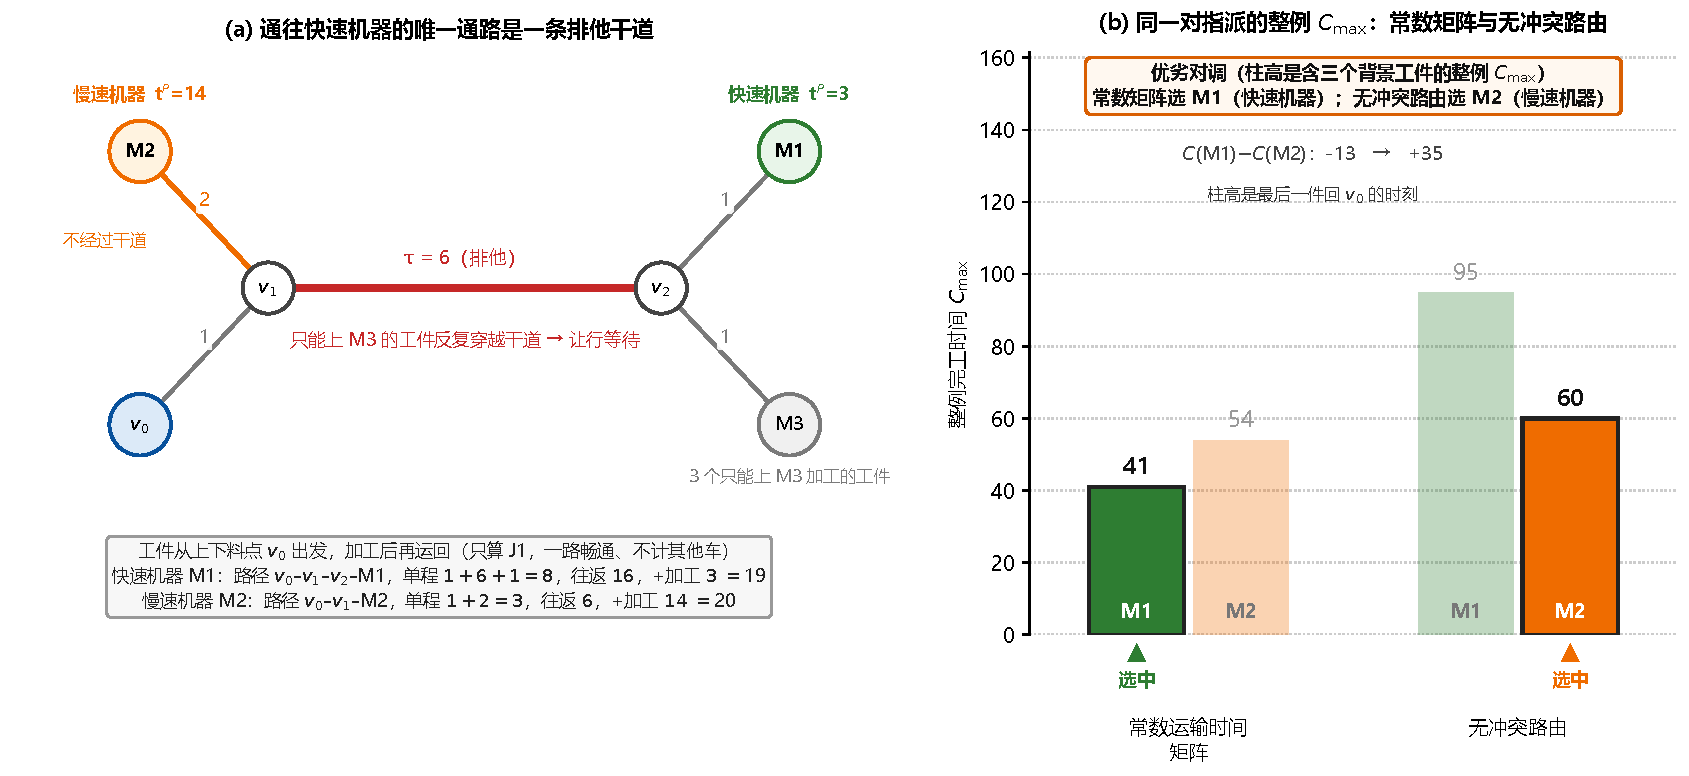
\includegraphics[width=\textwidth]{fig/fig_motivating_CN.pdf}
\Description{两幅。左图是小型车间网络：通往快速机器的唯一通路经过排他干道，慢速机器挂在自有支路上，底部写出焦点工件的畅通往返时间 19 对 20。右图是同一对指派的整例完工时间：常数矩阵下快速机器以 41 对 54 胜出，无冲突路由下变为 95 对 60、慢速机器胜出。}
\caption{动机算例：同一指派决策在两种评价下给出相反的选择。
(a) 通往快速机器 M1 的唯一通路是排他干道（$\tau=6$），慢速机器 M2 位于不经过干道的支路上；三个只能在 M3 上加工的工件反复穿越干道。
底部为焦点工件 J1 的畅通往返时间（M1：$19$；M2：$20$）。
(b) 柱高为整例完工时间 $C_{\max}$（$4$ 个工件、$2$ 辆 AGV，与正文相同的解码器）。
按常数运输时间评价为 $41$ 对 $54$，选快速机器；按无冲突路由评价为 $95$ 对 $60$，选慢速机器。
时间均为无量纲时间单位。在围绕该算例的 $1200$ 组参数中，有 $205$ 组（$17\%$）出现这种反转。}
\label{fig:motivating}
%% 由 fig/fig_motivating_CN.py 从 clbs/output/motivating.json 生成,后者由
%% clbs/tools/motivating.py --sweep 用与论文同一套解码器算出((b) 的四个数不是示意值:
%% 理想矩阵 = decode(conflict_free=False),无冲突路由 = decode(conflict_free=True))。
%% 算例:4 工件 / 3 加工机器 / 6 节点 / 5 走廊 / 2 AGV,delta_return=1,规则派车。
\end{figure*}

\subsection{现有工作存在的问题}

贴近实际的 AGV 车间同时具备三个特征：工序可选机器且加工时间随机器而变；AGV 在单车道走廊上行驶，运输时间由各车路径共同决定；AGV 之间无冲突。针对这类车间，现有工作存在三个问题。

\textbf{(1) 运输时间按常数处理。} 带运输时间的柔性作业车间调度以常数矩阵表示运输~\cite{xin2025review,meng2025cp,qin2026knowledge}。这样排出的计划在单车道走廊上执行时会因让行而延误，常数矩阵下更优的指派实际可能更差（图~\ref{fig:motivating}）。

\textbf{(2) 路由与排产相互割裂。} 无冲突路径规划与派车的研究~\cite{gao2023mapf,zhang2024guidance,kim2026congestion}把运输任务视为给定，只能被动避让。两阶段方法先排产、后消解冲突~\cite{sun2023integrated}，或把路由得到的运输时间回传一次而不修改指派~\cite{li2026framework}。它们都无法通过改派机器从源头减少争用。

\textbf{(3) 联合优化缺少对收益与代价的度量。} van Os 与 Basten~\cite{vanos2026exact}以基于逻辑的 Benders 分解求至可证最优，但只适用于小规模算例。
Lyu 等~\cite{lyu2019approach}与贺长征等~\cite{he2019integrated}在遗传算法的解码中嵌入时间窗 Dijkstra，使每个候选解都按路由后的完工时间评价；但二者把 AGV 编入染色体随机搜索，冲突按局部规则消解，也未与开环排产对比，未报告嵌入路由的计算代价。
嵌入路由会使单次评价开销增加一个数量级以上，在固定算力下可完成的评价次数随之减少。因此，这样做能否降低完工时间，必须在相同算力下度量。

本文聚焦于上述工作未专门研究的一类车间：运输耗时超过加工（$\bar{T}_t/\bar{T}_p\approx4.0$，常用公开算例最高仅 \PubTtTpHi{}），拥堵集中在少数共享走廊上。
走廊排他与 AGV 相互阻塞在实际车间中已有报道：在以 AGV 连接分散工作站的矩阵式生产车间中，AGV 须先获得相邻路口间走廊的通行许可，以免相向行驶；AGV 增加到一定数量后，完工时间不再缩短，等待时间却持续上升~\cite{hardai2025matrix}。
运输耗时超过加工是本文为使争用成为主要约束而设定的受控条件；运输不超过加工的情形，本文实验未覆盖（第~\ref{sec:limitations}~节）。

\subsection{本文的主要思想与贡献}

本文的主要思想是：让无冲突路由的结果直接参与排产决策，并把由此增加的计算开销降到在相同算力下付得起。
为此，本文提出闭环双层框架（第~\ref{sec:Chapter_IV}~节）：上层用文化基因算法搜索机器指派与工序顺序；解码器按工序顺序逐个生成运输任务并选派 AGV；下层用时间窗 Dijkstra 在走廊预约表上为 AGV 规划无冲突路径。路由结果以两种方式进入决策：
\begin{itemize}[leftmargin=*,topsep=2pt,itemsep=1pt]
  \item \emph{路由内嵌评价}：每个候选解的适应度取为完成全部无冲突路由后的完工时间，让行等待因此直接进入搜索目标；
  \item \emph{预约表感知派遣}：为每个运输任务在当前预约表上试算各 AGV 的送达时刻，选实际最早者，而非按畅通行驶时间估计选车。
\end{itemize}
下文把采用路由内嵌评价的方法称为\emph{闭环}，把搜索时不计冲突、只在执行时路由的方法称为\emph{开环}。

本文的主要贡献如下：
\begin{enumerate}[leftmargin=*]
\item \textbf{问题与算例。} 研究走廊排他条件下柔性作业车间调度与 AGV 无冲突路由的一体化问题，构造争用强度可控的算例族，用于考察快、慢机器之间的改派权衡。

\item \textbf{方法。} 提出闭环双层框架，以路由内嵌评价与预约表感知派遣两项技术让路由结果进入排产；证明任意染色体都可解码为无冲突、无死锁的时间表，搜索中无需修复算子；提出下界剪枝与胜者路径复用两项加速，证明二者不改变所选 AGV 与时间表，并使派遣的单次评价开销由规则派车的 \CostMultBefore{} 倍降至 \CostMultAfter{} 倍。

\item \textbf{实验验证。} 以开环方法为起点构造四级基线，每级只改变一项机制，在相同挂钟时间预算下分别度量两项技术的收益：路由内嵌评价是主要来源（\GainLoopRule{}），预约表感知派遣是次要来源（\GainProbeLoop{}），二者不能互相替代。
\end{enumerate}

本文其余部分安排如下：第~\ref{sec:Chapter_II}~节综述相关工作；第~\ref{sec:Chapter_III}~节给出问题描述与数学模型；第~\ref{sec:Chapter_IV}~节介绍闭环双层框架；第~\ref{sec:Chapter_V}~节为实验与结果分析；第~\ref{sec:Chapter_VI}~节总结全文。全文符号汇总于表~\ref{tab:notation}。

\section{相关工作}
\label{sec:Chapter_II}

按所优化的决策，相关工作可分为三类：运输时间固定、只优化机器指派与工序顺序的柔性作业车间调度（第~\ref{sec:rw_fjsp}~节）；运输任务给定、只优化 AGV 路径与派车的研究（第~\ref{sec:rw_route}~节）；同时优化二者的一体化研究（第~\ref{sec:rw_integ}~节）。表~\ref{tab:related} 从问题设定与评价方式两方面对照了各类工作与本文。

\subsection{考虑运输的柔性作业车间调度}
\label{sec:rw_fjsp}

带运输时间的柔性作业车间调度（FJSP\_PT）把工件在机器之间的搬运纳入排产。Xin 等~\cite{xin2025review} 的综述指出，该领域的主流建模方式是常数运输时间矩阵：AGV 从 $a$ 到 $b$ 的耗时固定为 $t(a,b)$，不考虑 AGV 之间的路径冲突与让行等待。综述还指出，这类假设「会降低问题复杂度，甚至改变问题的性质」；现有算例「主要在规模上有差别，缺少针对关键问题参数取值的专门设计」；平均运输与加工时间之比 $\bar{T}_t/\bar{T}_p$ 很可能影响算法表现。
% [ref_check: key=xin2025review; claim="该综述覆盖至 2023 年的进展,并将求解方法分为精确/启发式/元启发式/群智能四类"; need=quote]
% [ref_check: key=xin2025review; claim="常数行驶时间矩阵是 FJSP_PT 文献中占主导地位的建模约定"; need=quote]
% [ref_check: key=xin2025review; claim="该综述把常数行驶时间矩阵本身列为局限性建模选择而非已成定论"; need=quote]
% [ref_check: key=xin2025review; claim="该综述把平均运输时间与平均加工时间之比列为极可能影响算法表现的参数,并呼吁扩充测试集"; need=quote]

近年工作沿用常数矩阵，主要改进求解方法。Meng 等~\cite{meng2025cp} 提出约束规划模型与约束规划辅助的双种群遗传算法，关闭了 29 个开放基准算例，并改进了 27 个最优已知解；Qin 等~\cite{qin2026knowledge} 结合质量--多样性存档与 Q 学习，并设计了由 AGV 与关键路径共同制导的局部搜索；Jafarian-Moghaddam 等~\cite{jafarian2026integrated} 研究 U 形柔性流水车间排产与内部物流的联合优化。
这些工作的运输时间都取自矩阵，AGV 之间不会因争用走廊而相互推迟，因而会出现图~\ref{fig:motivating} 所示的误判。此外，关键链推理是作业车间局部搜索的成熟手段~\cite{otala2021graph,tamssaouet2023neighborhood}，但在常数矩阵上算出的关键路径只能追溯到前驱工序或机器繁忙，无法定位到具体走廊。
% [ref_check: key=meng2025cp; claim="关闭 29 个此前开放的基准算例并改进 27 个最优已知解"; need=quote]
% [ref_check: key=meng2025cp,qin2026knowledge,jafarian2026integrated; claim="三者的运输时长均取自常数矩阵,车辆之间不产生相互延误"; need=quote]

\subsection{任务给定的无冲突路由与派车}
\label{sec:rw_route}

这类工作只决定 AGV 的路径与派车，运输任务的起点、终点与释放时刻由外部给定；本文下层的路由与派遣即属于这一类问题。
多智能体路径规划（MAPF）研究多个智能体在共享图上的无碰撞行驶，其最优求解为 NP 难~\cite{gao2023mapf}；Kasaura 等~\cite{kasaura2022sipp} 把安全区间规划推广到二维路网与连续时间。
Zhang 等~\cite{zhang2024guidance} 针对任务持续到达的设定，离线优化一张带边权的路网，把智能体从瓶颈处引开。Kim 与 Kim~\cite{kim2026congestion} 为大规模 AGV 车队提出拥堵函数、拥堵惩罚与拥堵感知的派车规则。
多 AGV 管理与移动机器人控制的综述~\cite{lu2022agv,fragapane2021planning} 把派遣与路径规划列为控制栈上相邻而独立的两层，空闲优先与最近车辆是常用的单属性派遣规则。
这类工作有两点局限：一是路由器无法修改产生运输任务的机器指派；二是拥堵多用局部车辆密度或离线边权等间接指标刻画，只能说明某条走廊车辆偏多，不能指明哪次运输在何时、何处造成了让行。
% [ref_check: key=zhang2024guidance; claim="制导图抑制迎面运动并提升多个终身式求解器的吞吐"; need=quote]
% [ref_check: key=zhang2024guidance,kim2026congestion; claim="两者的任务释放时刻与起终点均为外生输入,路由器不参与任务生成"; need=quote]
% [ref_check: key=kim2026congestion; claim="其拥堵度量为局部车辆密度"; need=quote]
% [ref_check: key=zhang2024guidance; claim="其制导图边权为离线学得而非在线更新"; need=quote]

\subsection{调度与无冲突路由的一体化}
\label{sec:rw_integ}

同时考虑机器指派与无冲突路由的工作较少。按路由结果如何进入排产，可分为三种。

\textbf{(1) 精确分解。} van Os 与 Basten~\cite{vanos2026exact} 提出基于逻辑的 Benders 分解：约束规划主问题给出指派与顺序，整数规划子问题规划无冲突路径，并把冲突作为割回传。多数基准算例被求至可证最优，但该方法只适用于小规模算例。作者指出，如何更充分地利用「不可行由哪些冲突造成」的信息来指导主问题，有待研究。

\textbf{(2) 先排产、后路由。} Sun 等~\cite{sun2023integrated} 先用混合遗传算法确定指派与顺序，再用时间窗 Dijkstra 依次为各运输任务规划路径；第二阶段即使发现走廊拥堵，也只能靠等待消解，无法改动第一阶段的指派。Li 等~\cite{li2026framework} 加入一次反馈，把路径层的运输时间写回时间轴，但反馈只平移开工时刻、不修改指派，且其基准中每道工序只有一台可选机器。

\textbf{(3) 解码内嵌路由。} Lyu 等~\cite{lyu2019approach} 与贺长征等~\cite{he2019integrated} 把时间窗 Dijkstra 嵌入遗传算法的解码，每个染色体都在无冲突路由之后计算完工时间。二者都把 AGV 编入染色体（工序、机器、AGV 三段式编码），靠交叉与变异搜索；路口、相向与节点占用等冲突按局部规则以等待或绕行消解。Lyu 等的研究重点是确定最优车队规模；贺长征等提出求解集成调度的混合遗传算法，主要在非柔性算例上与文献报告值比较。二者都未与开环排产对比，也未报告嵌入路由的计算代价，因此无法据此判断：在相同算力下，把路由嵌入评价是否值得。
% [ref_check: key=vanos2026exact; claim="多数基准算例求至可证最优,约半数相对既有启发式改进完工时间不少于 10%"; need=quote]
% [ref_check: key=sun2023integrated; claim="第二阶段的冲突消解不反馈修改第一阶段的排程与指派"; need=quote]
% [ref_check: key=li2026framework; claim="其反馈内容仅为时间,且实验基准为每工序单一可选机器"; need=quote]
% [ref_check: key=lyu2019approach; claim="GA 解码内嵌时间窗 Dijkstra;研究重点为车队规模;未与开环排产对比"; need=quote]

\subsection{小结}

由表~\ref{tab:related} 可见，已有工作的差别不在于是否处理 AGV 冲突，而在于路由结果如何进入排产，以及这样做的收益与代价。
与最接近的解码内嵌路由工作~\cite{lyu2019approach,he2019integrated}相比，本文在机器异构、走廊排他与评价方式上相同（表中第 3--5 列），区别有三点：
\begin{enumerate}[label=(\arabic*),leftmargin=*,topsep=2pt,itemsep=1pt]
  \item \emph{研究问题不同}：本文不以提出更强的求解算法为目标，而是在运输耗时超过加工、拥堵集中于少数走廊的车间中，度量把路由纳入排产能降低多少完工时间、需付出多少计算代价；
  \item \emph{方法不同}：AGV 不编入染色体，而在解码时按预约表试算选派，并以两项可证明不改变结果的加速降低开销；路由在当前预约表下可证最早到达，任意解可证无冲突、无死锁；
  \item \emph{验证方式不同}：以每次只改变一项机制的基线，在相同挂钟时间预算下做多种子配对检验，把收益分别归因于路由内嵌评价与预约表感知派遣。
\end{enumerate}
建模上，本文只把走廊作为排他资源、在节点设停靠位，而上述两项工作的节点也排他（第~\ref{sec:fjsppt}~节）；这是建模选择的不同，不构成优劣。

\begin{table}[t]
  \caption{相关工作与本文的对照。「机器异构」：一道工序有多台可选机器且加工时间随机器而变。「走廊排他」：一条走廊任一时刻至多容一辆 AGV。「排产评价所用运输时长」：上层比较候选排产时所用的运输时间，「畅通估计」为不计其他 AGV 的最短路时间，「路由实算」为完成无冲突路由后、含让行等待的时间。「度量闭环收益与代价」：是否在相同算力下、相对开环度量了把路由纳入搜索评价的收益与计算开销。}
\label{tab:related}
%% 手工维护表:无生成脚本;任一行改动须同步 §2.3 正文。与 tab/ 下由 gen_tables_ladder.py 生成的表区分。
\footnotesize
\renewcommand{\arraystretch}{1.2}
\begin{tabular}{@{}p{2.3cm}cccp{2.7cm}cp{2.9cm}@{}}
\toprule
工作类别 & 文献 & 机器异构 & 走廊排他 & 排产评价所用运输时长 & \begin{tabular}[t]{@{}c@{}}度量闭环\\收益与代价\end{tabular} & 研究重点 \\
\midrule
FJSP\_PT 元启发式 & \cite{meng2025cp,qin2026knowledge,jafarian2026integrated}
  & 有 & 否 & 畅通估计（常数矩阵） & 否 & 常数矩阵下改进求解质量 \\
终身式 MAPF & \cite{gao2023mapf,zhang2024guidance}
  & --- & 是 & 无排产（任务外生） & 否 & 任务持续到达时的路网吞吐 \\
拥堵感知派车 & \cite{kim2026congestion}
  & --- & 否 & 无排产（任务外生） & 否 & 大规模车队的拥堵缓解 \\
两阶段 FJSP + 路由 & \cite{sun2023integrated}
  & 有 & 是 & 畅通估计；排产冻结后再路由 & 否 & 先排产、后消解冲突 \\
强化学习调度 + PBS & \cite{li2026framework}
  & 无 & 是 & 畅通估计；事后一次修正 & 否 & 强化学习排产与多车路径的分层框架 \\
GA 内嵌时间窗路由 & \cite{lyu2019approach,he2019integrated}
  & 有 & 是 & 路由实算（每个候选解）；AGV 编入染色体 & 否 & 最优车队规模~\cite{lyu2019approach}；AGV 与机器集成调度算法~\cite{he2019integrated} \\
精确分解（LBBD；限小规模） & \cite{vanos2026exact}
  & 有 & 否 & 松弛下界 + 冲突割 & 否 & 小规模可证最优 \\
\textbf{本文} &
  & 有 & 是 & \textbf{路由实算（每个候选解）}；派车按预约表试算 & \textbf{是（同挂钟）} & \textbf{走廊争用下快慢机器的改派权衡；相同算力下闭环的收益与代价} \\
\bottomrule
\end{tabular}
\end{table}


\section{问题描述与数学模型}
\label{sec:Chapter_III}

\subsection{问题描述}

一个算例包含 $n$ 个工件、$N_M$ 台加工机器与 $N_A$ 辆 AGV，它们在一个以图表示的车间路网中运行。工件 $j$ 有固定的工序链 $O_{j1}\to\cdots\to O_{jn_j}$；工序 $O_{ji}$ 可在其可选集 $\Omega_{ji}\subseteq M$ 中的任一机器上加工，在机器 $m$ 上的加工时间为 $t^P_{jim}$。机器位于图中的固定节点，工件由 AGV 在这些节点之间搬运。问题要求同时确定以下四组决策，使完工时间 $C_{\max}$ 最小：

\begin{enumerate}[label=(\roman*),leftmargin=*,topsep=2pt,itemsep=1pt]
\item 机器指派：为每道工序 $O_{ji}$ 选择一台机器 $m\in\Omega_{ji}$；
\item 工序排序：确定每台机器上各工序的加工顺序；
\item AGV 指派：把由此产生的运输任务分配给 AGV，并确定每辆 AGV 的任务顺序；
\item 路由：为每一次 AGV 行驶规划路径，要求时间与空间上无冲突，允许等待。
\end{enumerate}
主要符号见表~\ref{tab:notation}。

\begin{table}[t]
\caption{符号说明。}
\label{tab:notation}
\small
\begin{tabular}{@{}ll@{}}
\toprule
符号 & 含义 \\
\midrule
$J=\{1,\dots,n\}$, $O_{ji}$ & 工件集合；工件 $j$ 的第 $i$ 道工序，$i\le n_j$ \\
$M=\{1,\dots,N_M\}$, $\Omega_{ji}\subseteq M$ & 加工机器集合；$O_{ji}$ 的可选加工机器集 \\
$t^P_{jim}$ & $O_{ji}$ 在加工机器 $m\in\Omega_{ji}$ 上的加工时间 \\
$K=\{1,\dots,N_A\}$ & 同构的单载量 AGV \\
$G=(V,E)$, $\tau_e$ & 车间路网（顶点：上下料点、机器节点与路口；边：走廊）；走廊 $e$ 的通行时间 \\
$v_0$, $\mathrm{loc}(m)$ & 上下料点；加工机器 $m$ 所在节点 \\
$t^{*}(a,b)$ & $G$ 中 $a$ 到 $b$ 的最短路时间，不计争用 \\
$\delta_{\mathrm{ret}}\in\{0,1\}$ & 完工工件是否返回 $v_0$(基准取 $1$) \\
$S_{ji}$, $C_{ji}$, $A_{ji}$ & $O_{ji}$ 的开工、完工与物料到达时刻 \\
$C_{\max}$ & 完工时间 \\
\bottomrule
\end{tabular}
\end{table}

\subsection{建模假设}
\label{sec:assumptions}

\begin{enumerate}[label=\textbf{A\arabic*.},leftmargin=*,topsep=2pt,itemsep=2pt]
\item \textbf{静态与完全信息。} 全部工件在 $t=0$ 时位于 $v_0$，不设释放时刻与交货期；加工数据、路网 $G$ 与 AGV 状态在规划时已知。

\item \textbf{工件。} 每个工件有固定的工序链；加工与运输均不可抢占，工件不可拆分，不同工件之间没有外生的先后约束。

\item \textbf{加工机器：部分柔性且工时异构。} 多数工序满足 $|\Omega_{ji}|\ge 2$，完全柔性 $\Omega_{ji}=M$ 是其特例。加工时间随机器而变，且各机器之间不要求有统一的快慢关系（$t^P_{jim}$ 与 $t^P_{jim'}$ 不必成比例）。一台机器同时只加工一道工序，计划期内不发生故障，准备时间并入 $t^P_{jim}$。

\item \textbf{缓冲区与装卸。} 各机器的输入、输出缓冲区及 $v_0$ 的存储容量充裕，不发生阻塞；装卸时间可忽略，且不占用机器。

\item \textbf{AGV。} $N_A$ 辆 AGV 同构、单载量，以恒定速度行驶，不建模加减速与电量；$t=0$ 时全部空载停于 $v_0$。运输任务是一次单程搬运，共三类：从 $v_0$ 到第一台机器；在前后两台不同的机器之间；当 $\delta_{\mathrm{ret}}=1$ 时从最后一台机器返回 $v_0$。任一 AGV 可执行任一任务，同一工件的连续搬运可由不同 AGV 接力；卸货后 AGV 不必返回 $v_0$，其出发时刻可由路由推迟。

\item \textbf{路网与无冲突。} 路网 $G=(V,E)$ 强连通：顶点为 $v_0$、各机器所在节点与路口，每条边 $e$ 是一条可双向通行的单车道走廊，通行时间 $\tau_e$ 为已知常数。走廊是\emph{排他}资源：两个方向共享同一份预约，任一时刻至多一辆 AGV 占用 $e$，从而排除迎面冲突与同向超车。占用区间取半开形式 $[t,\,t+\tau_e)$，后一辆 AGV 可恰在 $t+\tau_e$ 进入。节点设有容量充裕、与通行资源独立的停靠位，等待总是允许的。

\item \textbf{不在建模范围内。} 机器与 AGV 故障、有限缓冲与阻塞、充电，以及工件动态到达（已有专门研究~\cite{gui2023dynamic,zhao2026deep}），留待后续工作（第~\ref{sec:future_work}~节第 (5) 条）。
\end{enumerate}

其中 A1、A2、A4、A5 是 FJSP\_PT 文献中的标准假设~\cite{xin2025review}。决定本文问题特征的是 A3 与 A6：A3 使机器选择成为加工时间与运输时间之间的权衡；A6 把争用表述为显式的排他资源约束，使运输时间不再是常数，而是路由决策的结果。
无死锁不作为假设：第~\ref{sec:upper}~节命题~\ref{prop:decodable} 基于 A4 与 A6 证明，任意指派与工序顺序都可解码为无冲突、无死锁的时间表。

\subsection{运输任务与决策变量}

令 $x_{jim}\in\{0,1\}$ 表示工序 $O_{ji}$ 指派给机器 $m$，记 $\mathrm{m}(j,i)$ 为所选机器，$d_{ji}=\mathrm{loc}(\mathrm{m}(j,i))$ 为其所在节点。当 $\delta_{\mathrm{ret}}=1$ 时，为每个工件追加一道位于 $v_0$、加工时间为零的\emph{伪工序} $O_{j,n_j+1}$，表示完工后返回上下料点；这样，返回与中间搬运使用同一套记号。

与车辆路径问题不同，运输任务不是输入，而是由机器指派\emph{派生}的：
\begin{equation}
\label{eq:tasks}
\mathcal{T}(x)=\Bigl\{\,(j,i)\ :\ d_{j,i-1}\neq d_{ji}\,\Bigr\},
\qquad d_{j0}\equiv v_0 ,
\end{equation}
任务 $(j,i)$ 把工件 $j$ 从 $d_{j,i-1}$ 搬到 $d_{ji}$，就绪时刻为 $r_{ji}=C_{j,i-1}$（约定 $C_{j0}=0$）。前后两道工序在同一台机器上时不产生运输任务。因此，运输任务的\emph{数量}与\emph{起止节点}都由机器指派决定：工件始终留在同一台机器上只需搬运两次，每道工序都换机器则需搬运 $n_j+1$ 次。
任务到 AGV 的指派用 $y_{tk}\in\{0,1\}$ 表示，对每个 $t\in\mathcal{T}(x)$ 有 $\sum_{k\in K}y_{tk}=1$，分给同一辆 AGV 的任务排成一条先后次序。
在常数运输时间模型中，指派同样决定搬运的次数与起止节点；本文中，它还决定这些搬运会在哪些走廊上相互争用。

\subsection{约束与目标}

记 $p_{ji}=\sum_{m\in\Omega_{ji}}x_{jim}t^P_{jim}$ 为所选机器上的加工时间。指派、工序时长、物料到达与机器容量约束为
\begin{align}
\sum_{m\in\Omega_{ji}} x_{jim} &= 1, & \forall j,i,
\label{eq:assign}\\
C_{ji} &= S_{ji}+p_{ji}, & \forall j,i,
\label{eq:dur}\\
S_{ji} &\ \ge\ A_{ji}, & \forall j,i,
\label{eq:material}\\
S_{j'i'}\ \ge\ C_{ji}\ \ \vee\ \ S_{ji} &\ \ge\ C_{j'i'}
& \forall (j,i)\neq(j',i')\ \text{位于同一加工机器},
\label{eq:disj}
\end{align}
其中 $A_{ji}$ 是工件 $j$ 到达 $d_{ji}$ 的时刻。若 $(j,i)\notin\mathcal{T}(x)$，工件本已在该处，$A_{ji}=C_{j,i-1}$；否则 $A_{ji}$ 由承运任务 $(j,i)$ 的 AGV 决定。记 $a^{\mathrm{E}}_{ji}$ 为该 AGV 经空载段到达取货节点的时刻，则
\begin{equation}
\label{eq:load}
\ell_{ji}=\max\bigl(a^{\mathrm{E}}_{ji},\ r_{ji}\bigr),
\qquad
A_{ji}=\text{于 } \ell_{ji} \text{ 出发的满载段的到达时刻},
\end{equation}
即 AGV 可以等工件，工件也可以等 AGV。空载段与满载段都是 $G$ 中的一条通路 $(e_1,\dots,e_q)$，其走廊进入时刻 $\eta_1,\dots,\eta_q$ 满足
\begin{equation}
\label{eq:walk}
\eta_1 \ \ge\ \sigma, \qquad
\eta_{l+1}\ \ge\ \eta_l+\tau_{e_l}, \quad l=1,\dots,q-1,
\end{equation}
其中 $\sigma$ 为该段可开始的时刻；$\eta_{l+1}>\eta_l+\tau_{e_l}$ 时，差额即在停靠位的让行等待。该段在 $\eta_q+\tau_{e_q}$ 结束。
走廊排他约束为：对同一走廊 $e$ 的任意两次不同占用，
\begin{equation}
\label{eq:excl}
\bigl[\eta,\ \eta+\tau_e\bigr)\ \cap\
\bigl[\eta',\ \eta'+\tau_e\bigr)\ =\ \emptyset ,
\end{equation}
与方向和所涉 AGV 无关。它是模型中唯一通过\emph{空间}（而非共享机器）把不同工件耦合起来的约束。目标函数为
\begin{equation}
\label{eq:obj}
\min\ C_{\max},\qquad
C_{\max}=\max_{j\in J}\ C_{j,\,n_j+\delta_{\mathrm{ret}}} .
\end{equation}

在半活动排程中（每道工序在约束允许的最早时刻开工），式~\eqref{eq:material} 与式~\eqref{eq:disj} 收紧为
\begin{equation}
\label{eq:bind}
S_{ji}=\max\bigl(A_{ji},\ F_{\mathrm{m}(j,i)}\bigr),
\end{equation}
其中 $F_m$ 是机器 $m$ 上前一道工序的完工时刻，即开工时刻取工件到达与机器空闲中的较晚者。第~\ref{sec:Chapter_IV}~节据此把一次开工推迟追溯为待料或待机器。

\subsection{与 FJSP\_PT 及已有冲突模型的关系}
\label{sec:fjsppt}

去掉式~\eqref{eq:excl} 后，各段行驶不再相互占用走廊，每段都可以沿最短路不停顿地行驶，运输时间退化为常数矩阵 $t^{*}(a,b)$，模型即成为 FJSP\_PT。$t^{*}$ 在后文用作下界，也在开环基线中用于估计到达时刻。

与同样给出显式路网的工作相比，区别在于把哪种资源视为被争用的资源。van Os 与 Basten~\cite{vanos2026exact} 预约\emph{节点}：两辆 AGV 不得同时占据同一节点，也不得交换节点。Lyu 等~\cite{lyu2019approach} 与贺长征等~\cite{he2019integrated} 走廊双向排他，同时限定每个节点只容一辆 AGV。本文只预约\emph{走廊}，在节点设容量充裕的停靠位，与 A4 对缓冲区的处理一致，对应实际车间中工位旁的待命区；拥堵因而只发生在走廊上。算例不能直接对比的原因见第~\ref{sec:limitations}~节局限 (1)。

\subsection{计算复杂度}

\begin{prop}
\label{prop:np_hard}
由式~\eqref{eq:assign}--\eqref{eq:obj} 定义的柔性作业车间与无冲突路由一体化调度问题是强 NP 难的；且当所有工序均满足
$\Omega_{ji}=M$ 时依然如此。
\end{prop}

\begin{proof}
限制到如下算例：对所有 $e\in E$ 有 $\tau_e=0$，每台加工机器各由一条专用走廊与 $v_0$ 相连，
且 $N_A=n$。此时每一段行驶耗时为零、占用的半开区间 $[t,t)=\emptyset$，故式~\eqref{eq:excl}
恒真，任何 AGV 都无法延误另一辆 AGV；又因每个工件独占一辆 AGV，式~\eqref{eq:load} 从不起作用，
$A_{ji}=C_{j,i-1}$。余下的正是取 $A_{ji}=C_{j,i-1}$ 的
式~\eqref{eq:assign}--\eqref{eq:disj}，也就是无关机器情形下的柔性作业车间调度问题。它的两个
特例已是强 NP 难的：处处取 $|\Omega_{ji}|=1$ 时退化为经典作业车间问题，在三台机器下即为
强 NP 难；取 $\Omega_{ji}=M$ 且 $n_j=1$ 时退化为无关并行机上
的完工时间最小化问题，它包含同型并行机调度，在机器数可变时为强 NP 难。
一般柔性作业车间调度本身即为强 NP 难~\cite{dauzereperes2024fjsp}。上述每个限制均为
多项式规约，故一般问题是强 NP 难的；第二个特例同时说明完全柔性并不会使问题变容易。
\end{proof}
该结论由已知结果直接规约得到，列出是为说明问题难度，不是本文的贡献。规约排除了 AGV 争用，说明即使没有走廊争用，问题已是强 NP 难；固定决策 (i)--(iii) 之后，余下的路由仍是一个无冲突多智能体路由问题~\cite{gao2023mapf}。小规模算例已有精确方法~\cite{vanos2026exact}，本文面向精确分解难以求解的规模。

\section{闭环双层框架}
\label{sec:Chapter_IV}

\subsection{主要思想与总体流程}
\label{sec:overview}

\paragraph{主要思想}
第~\ref{sec:Chapter_III}~节的四组决策中，机器指派与工序顺序决定运输任务的数量与去向，AGV 选择与路径决定每次运输实际耗时多少。开环方法先按畅通行驶时间确定前者、再规划后者，排产时看不到让行等待。
本文的思路是让路由结果反过来参与排产：每评价一个候选解，都先为其全部运输任务完成无冲突路由，再以所得完工时间评价它。为此，框架把四组决策分配到两层（图~\ref{fig:framework}）：
\begin{itemize}[leftmargin=*,topsep=2pt,itemsep=1pt]
  \item 上层用文化基因算法（遗传算法与局部搜索相结合~\cite{zhang2024memetic}）搜索机器指派与工序顺序；
  \item 解码器属于上层的适应度评价，它按工序顺序逐个生成运输任务，并为每个任务选派 AGV；
  \item 下层用时间窗 Dijkstra 在走廊预约表上为所选 AGV 规划无冲突路径。
\end{itemize}
框架的输入是一个算例：各工件的工序链、各工序的可选机器与加工时间、AGV 数量与走廊网络。输出是一张无冲突时间表（各工序的机器与起止时刻、各 AGV 的路径与走廊进入时刻）及其完工时间。

\paragraph{两项关键技术}
路由结果以两种方式进入决策，分别对应图~\ref{fig:framework} 中的两条反馈通路。
\begin{description}[leftmargin=0pt,topsep=3pt,itemsep=3pt]
  \item[路由内嵌评价（通路 1）。]
  每个候选解的适应度 $C_{\max}$ 取为下层完成全部运输任务的无冲突路由之后的完工时间，其中已含让行等待。它影响上层选择哪组机器指派与工序顺序，每个候选解回传一次。
  \item[预约表感知派遣（通路 2）。]
  解码时，为每个运输任务在当前预约表上试算各 AGV 的空载段与满载段，选实际送达最早的 AGV，而非按畅通行驶时间估计选车（第~\ref{sec:dispatch}~节）。它影响每个运输任务由哪辆 AGV 承运，每个任务试算一次。
\end{description}
两者作用于不同决策，不能互相替代：染色体不编码 AGV，路由内嵌评价无法改变选车；选车也无法改变机器指派。
预约表感知派遣使每个运输任务的路由调用从 $2$ 次增至至多 $2N_A$ 次，因此本文另给出两项可证明不改变结果的加速（第~\ref{sec:speedup}~节）。
上层的遗传算法与局部搜索采用常规设计，不是本文的贡献。

%% 本图由 fig/fig_framework_CN.py 生成,是一张示意图,不含任何数据。
%% 注意不要复用 fig/fig_hdp_architecture*.pdf,那是上一篇论文的 HDP 框架。
\begin{figure*}[t]
\centering
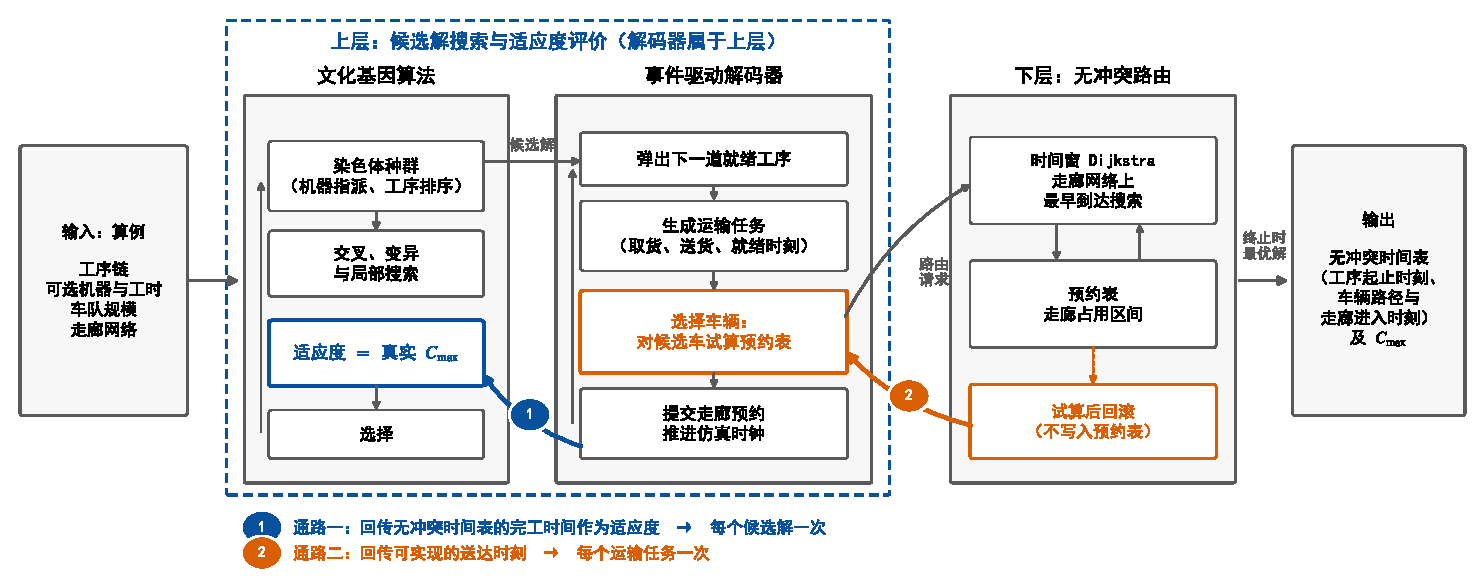
\includegraphics[width=\textwidth]{fig/fig_framework_CN.pdf}
\caption{闭环双层框架。上层包括文化基因算法与事件驱动解码器，解码器属于适应度评价过程；下层以时间窗预约做无冲突路由。
通路 1（蓝）：下层为全部运输任务完成无冲突路由后，把所得时间表的完工时间作为适应度回传，每个候选解一次。
通路 2（橙）：选派 AGV 前在预约表上试算空载段与满载段的最早送达时刻，每个运输任务一次，试算不写入最终时间表。}
\Description{Schematic of the closed-loop bilevel framework: an upper memetic
search layer, an event-driven decoder, and a lower time-window reservation
routing layer, with two colour-coded feedback paths entering the upper layer at
different places---the evaluation path returning a realized makespan once per
candidate, and the decision path returning a realizable arrival time once per
transport task.}
\label{fig:framework}
\end{figure*}

\paragraph{总体流程}
算法流程如下：
\begin{enumerate}[label={步骤\arabic*},leftmargin=3.6em,topsep=2pt,itemsep=1pt]
  \item \textbf{初始化。} 随机生成初始种群，并加入两个启发式个体（第~\ref{sec:ga}~节）。
  \item \textbf{解码与评价。} 对每个个体，按工序序列依次处理每道工序：若工件需要搬运，则生成运输任务，选定 AGV，再由下层为其规划空载段与满载段并写入预约表；随后计算该工序的开工与完工时刻。全部工序处理完后，以完工时间 $C_{\max}$ 作为该个体的适应度（第~\ref{sec:encoding}--\ref{sec:speedup}~节）。
  \item \textbf{局部搜索。} 对排名靠前的个体，按解码时记录的让行信息改派机器或调整顺序（第~\ref{sec:ls}~节）。
  \item \textbf{遗传操作。} 经选择、交叉与变异生成下一代种群（第~\ref{sec:ga}~节）。
  \item \textbf{终止判断。} 若挂钟时间预算用完或满足早停条件，输出最优个体的时间表；否则返回步骤2。
\end{enumerate}

\subsection{染色体编码}
\label{sec:encoding}

设工序总数为 $N=\sum_{j\in J}n_j$。一个染色体对应一个候选解，由两段组成：
\begin{itemize}[leftmargin=*,topsep=2pt,itemsep=1pt]
  \item \emph{机器指派向量}：长度为 $N$，按固定顺序列出所有工序，第 $k$ 个分量是第 $k$ 道工序所选机器的编号（取自其可选集 $\Omega_{ji}$）；该向量的下标次序不表示执行顺序。
  \item \emph{工序序列}：工件 $j$ 出现 $n_j$ 次，第 $x$ 次出现代表其第 $x$ 道工序 $O_{jx}$。序列给出全局先后，共用同一机器或同一走廊的工序按序列次序先后处理。
\end{itemize}
并行无需显式编码：解码时每道工序在其机器空闲且工件到达后即开工，不同机器上的加工、不同 AGV 的运输自然在时间上重叠。
当 $\delta_{\mathrm{ret}}=1$ 时，每个工件在序列中额外出现一次，对应第~\ref{sec:Chapter_III}~节的伪工序（地点固定为 $v_0$，加工时间为零），返回运输因此与中间运输按同一方式处理。

与把 AGV 编入染色体的三段式编码~\cite{lyu2019approach,he2019integrated}不同，本文不编码 AGV，而在解码时选派（第~\ref{sec:dispatch}~节）。原因有二：一是运输任务数随机器指派而变（式~\eqref{eq:tasks}），AGV 段长度不固定，交叉与变异后可能与实际任务不对应，需要修复算子；二是搜索空间约扩大 $N_A^{|\mathcal{T}(x)|}$ 倍。

\subsection{解码：从染色体到无冲突时间表}
\label{sec:upper}

解码器（算法~\ref{alg:decode}）把染色体转换为可执行的时间表并计算完工时间，是路由内嵌评价的实现。它自左向右扫描工序序列，维护三组状态：每台机器 $m$ 的空闲时刻 $F_m$（机器位于固定节点 $\mathrm{loc}(m)$）；每个工件 $j$ 的当前节点 $\mathrm{pos}_j$ 与就绪时刻 $\mathrm{ready}_j$；每辆 AGV $k$ 的当前节点 $\mathrm{loc}_k$ 与可用时刻 $\mathrm{avail}_k$。对每道工序 $O_{ji}$：
\begin{enumerate}[label=(\arabic*),leftmargin=*,topsep=2pt,itemsep=1pt]
  \item 若其机器所在节点与工件当前位置相同，不需搬运；
  \item 否则生成式~\eqref{eq:tasks} 的运输任务并选定一辆 AGV（规则派车按式~\eqref{eq:rule}，预约表感知派遣见第~\ref{sec:dispatch}~节），然后在实时预约表上依次规划空载段（AGV 当前位置到取货点）与满载段（取货点到目的地），二者由式~\eqref{eq:load} 衔接；
  \item 按式~\eqref{eq:bind} 计算开工与完工时刻并更新状态；同时记录开工是由工件到达（待料）还是机器上一道工序完工（待机器）决定，供局部搜索与案例分析使用。
\end{enumerate}

\begin{algorithm}[t]
\caption{\textsc{Decode}：以完整无冲突仿真作为适应度}
\label{alg:decode}
\small
\begin{algorithmic}[1]
\Require 算例、路网、指派 $x$、工序序列
\Ensure 完工时间、时间表、逐走廊的让行统计量
\State 对所有加工机器置 $F_m\gets 0$；对所有工件置 $\mathrm{pos}_j\gets v_0$、
       $\mathrm{ready}_j\gets 0$
\State 对所有 AGV 置 $\mathrm{loc}_k\gets v_0$、$\mathrm{avail}_k\gets 0$；清空预约表
\ForAll{按序列次序取出的工序 $O_{ji}$(含伪工序)}
  \State $m\gets$ 在 $x$ 下 $O_{ji}$ 的加工机器；$d\gets \mathrm{loc}(m)$
  \If{$\mathrm{pos}_j=d$}
     \State $A_{ji}\gets \mathrm{ready}_j$ \Comment{同机器连续，不生成运输任务}
  \Else
     \State 选定 AGV $k$(第~\ref{sec:dispatch}~节)
     \State $a^{\mathrm{E}}\gets\textsc{Route}(\mathrm{loc}_k,\mathrm{pos}_j,
            \mathrm{avail}_k,R,\text{真})$;\ \ $\ell\gets\max(a^{\mathrm{E}},
            \mathrm{ready}_j)$ \Comment{空载段同样占用走廊}
     \State $A_{ji}\gets\textsc{Route}(\mathrm{pos}_j,d,\ell,R,\text{真})$;\ \
            $\mathrm{loc}_k\gets d$;\ \ $\mathrm{avail}_k\gets A_{ji}$
     \State 按走廊累计让行时间
  \EndIf
  \State 若 $F_m>A_{ji}$ 则 $\texttt{bind}\gets\texttt{machine}$，否则
         $\texttt{bind}\gets\texttt{arrive}$ \Comment{记录待机器或待料}
  \State $S_{ji}\gets\max(A_{ji},F_m)$;\ \ $C_{ji}\gets S_{ji}+p_{ji}$;\ \
         $F_m\gets C_{ji}$;\ \ $\mathrm{pos}_j\gets d$;\ \
         $\mathrm{ready}_j\gets C_{ji}$
\EndFor
\State \Return $C_{\max}=\max_{j,i} C_{ji}$、时间表与逐走廊的让行统计量
\end{algorithmic}
\end{algorithm}

解码具有确定性：预约按解码器生成任务的次序写入；时刻相同时，路由的标签队列以（到达时刻，节点标识）为键、仅当新到达严格更早时才更新，派遣按 AGV 编号升序扫描、保留首个严格更优者。
因此一个染色体总对应唯一一张时间表。第~\ref{sec:Chapter_V}~节按种子配对比较各配置，依赖这一点。

\begin{prop}[任何染色体都可解码]
  \label{prop:decodable}
  对任意机器指派与任意工序序列，算法~\ref{alg:decode} 均终止，并返回一张满足以下三点的时间表：(a) 无冲突，即同一走廊上任意两次占用的区间互不重叠（式~\eqref{eq:excl}）；(b) 无死锁，即不存在 AGV 之间的循环等待；(c) 完工时间有限。因此搜索中不必调用修复算子。
\end{prop}

\begin{proof}
  按编码方式，工序序列是各工件前后约束的一个拓扑序：工件的第 $x$ 次出现代表其第 $x$ 道工序，因此读取 $\mathrm{ready}_j$ 时该值已知。
  缓冲区充裕（A4）意味着工序不会因无处存放而阻塞，故工件一经到达，式~\eqref{eq:bind} 总给出有限开工时刻。
  每次 \textsc{Route} 调用都在有限时间内返回（第~\ref{sec:router}~节），且只占用预约表上尚未占用的时段，故式~\eqref{eq:excl} 由构造成立。
  无死锁同样由构造得到：走廊是唯一被争用的资源（A6），等待只发生在容量充裕的停靠位上、不占用走廊；已写入预约表的占用均在有限时刻结束，因此不存在 AGV 之间的循环等待。
  扫描共执行 $N+n\delta_{\mathrm{ret}}$ 次，每次在有限时刻上安排有限个事件。
\end{proof}

\subsection{无冲突路由：预约表与时间窗 Dijkstra}
\label{sec:router}

解码器每选定一辆 AGV，便调用本节的路由器为其规划路径；预约表感知派遣在选车时也调用它做试算。

\paragraph{预约表}
唯一被争用的资源是走廊（假设 A6），因此预约表以走廊为索引：每条走廊 $e$ 对应一个按时间排序的占用区间列表，每个区间 $[t,\,t+\tau_e)$ 记录占用该走廊的 AGV 与运输任务。AGV 每规划一段路径，便把途经各走廊的占用区间写入表中；后规划的 AGV 查询该表以避开已占时段。
该表支持四种操作：查询不早于某时刻的最早可行进入时刻；写入一次占用；撤销某任务的全部占用；保存当前状态并在试算后恢复。
节点不被预约：穿越节点耗时为零，等待发生在停靠位上，因此路由器与独立校验器都只检查走廊占用。

\paragraph{时间窗 Dijkstra}
基本思想是：在普通 Dijkstra 上，把走廊的边权从固定通行时间 $\tau_e$ 换成「等到该走廊空闲所需的时间 $+\tau_e$」，等待时长由预约表查询得到。每次调用为一段行驶（空载段或满载段）一次性规划从起点到终点的完整路径。
标签 $(u,t)$ 表示 AGV 最早在时刻 $t$ 到达节点 $u$ 并停在其停靠位上；搜索以到达时刻为代价，目标是最早到达终点（算法~\ref{alg:route}）。
考察从 $u$ 出发的走廊时，向预约表查询最早可行进入时刻 $t'\ge t$，间隔 $t'-t$ 即在 $u$ 的让行等待；式~\eqref{eq:walk} 中的等待因此由搜索直接给出。
一次解码内，已写入的路径不再撤销，AGV 按解码器生成任务的次序依次规划，后规划者避让先规划者。

\begin{lem}[每个节点只需保留最早到达标签]
\label{lem:label}
对给定 AGV 的一段行驶（某运输任务的空载段或满载段），每个节点只保留到达最早的标签，即可得到在当前预约表下该 AGV 最早到达终点的路径。
\end{lem}

\begin{proof}
  停靠位容量充裕且不占用通行资源（A6），因此一辆自时刻 $t$ 起停在 $u$ 的 AGV，只需继续等到 $s$，
  就能走出任何在时刻 $s>t$ 才到达 $u$ 的 AGV 所能走的后续路径。
  故更早到达的标签不会更差。
  又记 $R.\textsc{EarliestEntry}(e,t,\tau_e)$ 为预约表 $R$ 上不早于 $t$、且与走廊 $e$ 的已有占用不重叠的最早进入时刻。
  查询时刻越晚，尚且可行的进入时段只减不增，故走完走廊 $e$ 的时刻
  $t\mapsto R.\textsc{EarliestEntry}(e,t,\tau_e)+\tau_e$
  关于 $t$ 单调不减。
  搜索按到达时刻从小到大取出标签，终点第一次被取出时即为最早到达。
\end{proof}

因此用普通 Dijkstra 即可，不必像安全区间规划（SIPP）那样按可行时段分标签~\cite{kasaura2022sipp}；若再引入第二项指标（例如走廊时段附加代价），更早到达不再总是更好，须改用多标签搜索（第~\ref{sec:interface}~节）。

\begin{algorithm}[t]
  \caption{\textsc{Route}：无冲突的单段路径规划}
  \label{alg:route}
  \small
  \begin{algorithmic}[1]
  \Require 起点 $s$、终点 $g$、最早出发时刻 $t_0$、预约表 $R$、是否写入预约表的标志 \textit{commit}
  \Ensure 到达时刻与走廊占用区间的序列；若 \textit{commit} 为真，这些区间同时写入 $R$
  \State 将标签 $(s,t_0)$ 放入以（时间，节点标识）为键的优先队列
         \Comment{时刻相同时按节点标识决定先后，次序确定}
  \While{队列非空}
    \State 取出键最小的标签 $(u,t)$
    \If{$u=g$} \State 回溯得到各占用区间；若 \textit{commit} 为真则逐一写入 $R$；
         \Return 到达时刻 $t$ \EndIf
    \ForAll{自 $u$ 出发的走廊 $e=(u,v)$}
      \State $t_{\text{in}} \gets R.\textsc{EarliestEntry}(e,t,\tau_e)$
         \Comment{在 $u$ 的停靠位等到 $t_{\text{in}}$}
      \State 若 $t_{\text{in}}+\tau_e$ 严格早于 $v$ 的已有到达时刻，则更新标签 $(v,\ t_{\text{in}}+\tau_e)$
    \EndFor
  \EndWhile
  \State \Return 失败 \Comment{$G$ 强连通时不应发生，见正文}
  \end{algorithmic}
\end{algorithm}

预约次数有限、时间有界，且 $G$ 强连通，故路径总是存在：最坏情况下 AGV 一直等到已有占用全部结束，再按畅通最短路行驶。
单次调用的代价为 $O\bigl(|E|\,(W^{2}+\log|V|)\bigr)$：至多考察 $|E|$ 条走廊，每条枚举 $O(W)$ 个候选进入时刻、每个候选做一次 $O(W)$ 的重叠判定，再做一次 $O(\log|V|)$ 的堆操作，其中 $W$ 为每条走廊上预约区间数的均值。
若预约表改用支持对数时间查询的有序结构，复杂度可降至 $O\bigl(|E|(\log W+\log|V|)\bigr)$；本文实现采用线性扫描。

对空预约表在所有取货--送货节点对上运行同一搜索，即得到第~\ref{sec:Chapter_III}~节的畅通最短路矩阵 $t^{*}$。它用于开环配置的到达时刻估计、改派邻域的打分与两阶段基线的运输时间，也是第~\ref{sec:speedup}~节剪枝所用的下界。

\subsection{预约表感知派遣}
\label{sec:dispatch}

常用的规则派车按畅通最短路估计每辆 AGV 完成该任务的送达时刻，并选估计值最小者：
\begin{equation}
\label{eq:rule}
\mathrm{score}(k)=\max\bigl(\mathrm{avail}_k+t^{*}(\mathrm{loc}_k,\text{取货点}),\,
\mathrm{ready}_j\bigr)+t^{*}(\text{取货点},\text{目的地}).
\end{equation}
该式与 Li 等~\cite{li2026framework} 的空闲优先派车相同，也是多 AGV 派遣中的典型单属性规则~\cite{lu2022agv}。它不查预约表，因此可能选中几何上近、走廊却已被占用的 AGV。

预约表感知派遣改为在预约表上试算。每个运输任务包含两段：空载段从 AGV 当前位置到取货点，满载段从取货点到目的地（AGV 已在取货点时空载段为零）。对每个运输任务，按以下步骤选车：
\begin{enumerate}[label=(\arabic*),leftmargin=*,topsep=2pt,itemsep=1pt]
  \item 按 AGV 编号升序遍历候选 AGV $k$；
  \item 计算下界 $\mathrm{lb}(k)$（式~\eqref{eq:lb_dispatch}），若不早于当前最好送达时刻则跳过 $k$（启用剪枝时，第~\ref{sec:speedup}~节）；
  \item 保存预约表状态，先试算空载段并临时写入，再试算满载段，得到送达时刻 $\mathrm{est}(k)$；空载段须先临时写入，否则满载段感知不到这段占用，试算结果会偏早；
  \item 回滚预约表；若 $\mathrm{est}(k)$ 严格早于当前最好，则记 $k$ 为当前胜者并缓存其两段路径；
  \item 遍历结束后，把胜者的两段路径正式写入预约表（启用胜者路径复用时直接写入缓存路径，否则重新规划）。
\end{enumerate}
AGV 能力相同（假设 A5），差别只在当前位置与走廊占用，因此预约表上的争用可以直接决定选哪辆 AGV。
代价是试算使每个运输任务的路由调用从 $2$ 次增至至多 $2N_A$ 次，单次评价开销约为规则派车的 \CostMultBefore{} 倍。

\subsection{两项加速：下界剪枝与胜者路径复用}
\label{sec:speedup}

按相同\emph{代数}比较（同一算例与种子下两种派车各运行相同代数，见图~\ref{fig:protocols} 与第~\ref{sec:protocol}~节），预约表感知派遣比规则派车好 \GainProbeSameGen{}；但由于单次评价开销为后者的 \CostMultBefore{} 倍，在相同\emph{挂钟时间}下这一增益几乎被抵消。
因此需要在不改变任何选择结果的前提下降低开销。本节给出两项这样的加速。

\paragraph{下界剪枝}
无冲突路由只会因让行而更晚，不可能快于忽略争用的最短路。因此规则派车的估计式~\eqref{eq:rule} 是实际送达时刻的可采纳下界：
\begin{equation}
\label{eq:lb_dispatch}
\mathrm{lb}(k)=\max\bigl(\mathrm{avail}_k+t^{*}(\mathrm{loc}_k,\text{取货点}),\,
\mathrm{ready}_j\bigr)+t^{*}(\text{取货点},\text{目的地})\ \le\ \mathrm{est}(k),
\end{equation}
其中 $\mathrm{est}(k)$ 为对 AGV $k$ 做完整两段试算所得的最早送达时刻。若某辆 AGV 的下界已不早于当前最好的试算送达时刻，则无需再为它调用路由。

\paragraph{胜者路径复用}
试算结束后预约表被回滚，胜者的两段路径随之作废，随后又要在同一张（已恢复的）预约表上为胜者重新规划，造成两次冗余调用。由于路由是确定性的，重新规划的结果与试算时相同，因此可直接写入试算时缓存的路径。

\begin{prop}[两项加速不改变所选 AGV 与时间表]
  \label{prop:speedup_equiv}
  按 AGV 编号从小到大依次试算，且仅当某 AGV 的送达时刻严格早于当前最好时才更换胜者。
  在此规则下，加入式~\eqref{eq:lb_dispatch} 的剪枝与胜者路径复用之后，所选 AGV、写入预约表的占用以及最终时间表，与对每辆 AGV 都做完整两段试算时相同。
\end{prop}

\begin{proof}
  先看剪枝。设扫到 AGV $k$ 时，当前最好的试算送达为 $\mathrm{est}^{\ast}$。
  若 $\mathrm{lb}(k)\ge \mathrm{est}^{\ast}$，则由式~\eqref{eq:lb_dispatch} 有
  $\mathrm{est}(k)\ge\mathrm{lb}(k)\ge\mathrm{est}^{\ast}$，
  故 $k$ 的送达不可能严格更早，完整试算时也不会选中它；不为它调用路由，胜者不变。
  每次试算前保存预约表、试算后恢复，未调用路由的 AGV 不改写预约表，因而不影响其后各次查询。
  再看复用：胜者的两段路径是在同一张预约表状态下算出的，恢复后的表与随后正式写入时面对的状态相同；
  路由是确定性的，故写入缓存路径与重新规划后再写入，所得占用区间完全相同。
\end{proof}

两项加速合计带来 \SpeedupProbe{} 倍加速，路由调用减少 \RouteCallCut{}，单次评价开销由规则派车的 \CostMultBefore{} 倍降至 \CostMultAfter{} 倍。实验中二者作为一个整体开关度量（表~\ref{tab:prune}），不分别归因。
剪枝效果随车队增大而减弱，但在所测最大车队上仍减少 \RouteCallCutLo{} 的路由调用；车队超过某一规模后派遣的收益可能消失，以现有种子数尚不足以确定这一规模（第~\ref{sec:whichcongestion}~节）。

\subsection{遗传操作}
\label{sec:ga}

上层的全局搜索采用常规遗传算法，适应度即解码得到的完工时间：
\begin{itemize}[leftmargin=*,topsep=2pt,itemsep=1pt]
  \item \emph{初始化}：机器从 $\Omega_{ji}$ 中均匀随机选取，工序序列随机打乱；另加入两个启发式个体，一个把每道工序指派给其最快机器，一个按负载均衡贪心指派。
  \item \emph{选择}：锦标赛选择，并保留少量精英。
  \item \emph{交叉}：工序序列采用保持工件内次序的顺序交叉，机器指派向量采用均匀交叉。
  \item \emph{变异}：交换工序序列中的两个位置，或把一道工序改派到另一台可选机器。
\end{itemize}
超参数见第~\ref{sec:impl}~节。

\subsection{按让行记录的局部搜索}
\label{sec:ls}

局部搜索作用于每代排名靠前的个体，主批次的四个配置均以相同设置启用。它利用解码时记录的\emph{让行记录}生成邻域：路由器在让行发生时已知走廊、时段与先行占用该走廊的运输任务，解码器把每次让行保存为三元组（走廊，时段，先行运输）。让行记录不进入任何目标函数，只决定局部搜索改动哪些工序。

\paragraph{关键链追溯}
从决定完工时间的事件回溯得到一条关键链。链上同时包括工序与运输段，并为每一节标注类型（表~\ref{tab:attrib}）：满载段上的让行记为走廊占用；空载段按让行时间占该段耗时的比例、以 $0.5$ 为阈值，区分为「车辆」或「走廊」。只有走廊占用一类能给出具体的走廊、时段与先行运输，局部搜索使用的正是这一信息。关键链追溯也用于第~\ref{sec:casestudy}~节的案例分析。

\begin{table}[t]
  \caption{关键链上各节的标注，以及可采取的改动。
  只有走廊占用这一类带有具体的走廊与时段，也只有它能指明先行占用该走廊的运输。}
\label{tab:attrib}
\footnotesize
\begin{tabular}{@{}llp{2.55cm}@{}}
\toprule
标注 & 判定条件 & 补救手段 \\
\midrule
\texttt{operation} & 一道真实工序正占用其加工机器 & --- \\
\texttt{machine} & 待机器：被该机器上前一道工序阻塞
  & 重排序 \\
\texttt{upstream} & AGV 先到，物料尚未就绪 & 递归至 $O_{j,i-1}$ \\
\texttt{vehicle} & 物料已就绪、AGV 迟到，且延误中让行占比很小 & 更换 AGV \\
\texttt{corridor} & 在指定走廊、指定时段上发生让行 & 改派或错峰 \\
\bottomrule
\end{tabular}
\end{table}

\paragraph{两类算子与接受准则}
\emph{改派}：对关键链上至多 $L=5$ 道真实工序 $O_{ji}$（设其当前机器为 $m$），为每台其他可选机器 $m'\in\Omega_{ji}\setminus\{m\}$ 计算
\begin{equation}
\label{eq:reassign}
\mathrm{score}(m')=t^{*}\bigl(d_{j,i-1},\mathrm{loc}(m')\bigr)
+t^{P}_{jim'},
\end{equation}
即从上一道工序所在节点 $d_{j,i-1}$ 到 $m'$ 的畅通行驶时间与 $m'$ 上的加工时间之和，取得分最低的机器生成一个只改这一道指派的邻居。它允许以较长的加工换取较短、更通畅的路径，即本文关注的改派权衡。

\emph{错峰}：取链上最长的走廊占用一节，生成两个邻居：将被阻塞的工序在序列中提前，或将先行占用的工序推后。移动只交换不同工件的相邻出现，工件内次序不变，由命题~\ref{prop:decodable} 仍可解码。

邻域因此至多含 $L+2=7$ 个候选。按首次改进接受，至多三轮；每轮依当前解重新计算关键链，因为一次成功改动后关键链往往随之改变（算法~\ref{alg:ls}）。

\begin{algorithm}[t]
\caption{\textsc{ContentionGuidedSearch}：按让行记录的局部搜索}
\label{alg:ls}
\small
\begin{algorithmic}[1]
\Require 染色体 $c$ 及其解码结果 $r$
\Ensure 一个完工时间不劣于 $r.C_{\max}$ 的染色体及其解码结果
\For{$\textit{round}=1$ \textbf{到} $3$}
  \State $\mathcal{N}\gets\textsc{Reassign}(c,r)\ \cup\ \textsc{Stagger}(c,r)$
     \Comment{至多 $L+2$ 个邻居，均由让行记录指定}
  \State \textit{improved} $\gets$ \textbf{假}
  \ForAll{$c'\in\mathcal{N}$}
    \State $r'\gets\textsc{Decode}(c')$
    \If{$r'.C_{\max}<r.C_{\max}$}
      \State $c\gets c'$;\ \ $r\gets r'$;\ \ \textit{improved} $\gets$
             \textbf{真}；\ \ \textbf{跳出}
    \EndIf
  \EndFor
  \If{\textbf{非} \textit{improved}} \State \textbf{跳出} \EndIf
\EndFor
\State \Return $c,r$
\end{algorithmic}
\end{algorithm}

\subsection{另两种层间接口：附加代价与让行记录}
\label{sec:interface}

路由内嵌评价与派遣试算从下层读取的都是计入让行后的实际运输时间，但它不指明是哪一项决策造成了等待。为检验下层传递更丰富的信息能否进一步降低完工时间，本文另实现两种接口作为对照，结果见第~\ref{sec:pricing}~节。

\paragraph{走廊时段附加代价}
类比拉格朗日松弛中以影子价格协调资源的做法，为每个走廊--时段槽位 $(e,b)$ 设附加代价 $\pi(e,b)$，使路径规划最小化「到达时刻 $+\theta\cdot$所经槽位的附加代价之和」（$\theta\ge0$ 为唯一可调参数），改派时也计入所需通行的附加代价。本文实现了两种估计：扰动单个槽位容量后重解，以及每代刷新的低成本近似。
从机制上看，附加代价不提供新信息：争用造成的等待已经进入 AGV 的到达时刻，再经式~\eqref{eq:bind} 进入完工时间并被适应度计入，再附加代价等于重复计入同一延误。它的主要开销来自引理~\ref{lem:label}：引入第二项指标后，单标签 Dijkstra 须换成多标签 Pareto 搜索，无论附加代价是否为零，单次评价开销都随之增加。

\paragraph{让行记录}
让行记录只用于生成局部搜索的邻域（第~\ref{sec:ls}~节），不进入目标函数：下层仍最小化到达时刻，上层仍最小化完工时间，因此不存在重复计入延误的问题。

\subsection{复杂度与计算开销}

一次适应度评价处理 $N+n\delta_{\mathrm{ret}}$ 个事件。预约表感知派遣下每次运输至多 $2N_A$ 次路由调用，故每个个体的评价代价为 $O\bigl((N+n)\,N_A\,|E|\,(W^{2}+\log|V|)\bigr)$；规则派车不含因子 $N_A$。
两项加速不改变这一最坏界，实测使路由调用减少 \RouteCallCut{}（各组在 \RouteCallCutLo{}--\RouteCallCutHi{} 之间）。局部搜索对每个被选中的个体至多增加 $3\times(L+2)=21$ 次解码。

各配置的单次评价开销差别很大。阶梯批次实测为：开环 \MsOpen{}\,ms，闭环规则派车 \MsLoopRule{}\,ms，完整闭环 \MsLoopProbe{}\,ms，闭环约为开环的 $37$ 倍；在另一批附加代价扫描中，开启附加代价使单次评价从 \MsPricedRef{}\,ms 升到 \MsPriced{}\,ms，约再乘 $4.8$ 倍。
两批的绝对耗时不可直接比较，但两个倍数之积表明，开销最高与最低的配置相差约两个数量级。在固定预算下，单次评价越贵，可完成的评价次数越少，因此第~\ref{sec:Chapter_V}~节不按相同代数，而按相同挂钟时间比较。

命题~\ref{prop:decodable}、引理~\ref{lem:label} 与命题~\ref{prop:speedup_equiv} 保证的是正确性而非解的质量：每个候选解都可行，其评价与第~\ref{sec:Chapter_III}~节的冲突模型一致，两项加速不改变任何选择，确定性解码使求解过程可复现。与多数元启发式一样，解的质量没有理论界，由下一节的实验评估。

\section{实验与结果分析}
\label{sec:Chapter_V}

实验回答四个问题：(1) 路由内嵌评价（闭环）能降低多少完工时间？(2) 预约表感知派遣能再降低多少，它能否替代闭环，二者合用是否相互放大？(3) 这些收益在哪些算例上成立，以现有种子数能否确定其范围？(4) 已实现但没有净收益的其他接口，失效原因是什么？各问题对应的实验见表~\ref{tab:plan}。

\begin{table}[t]
\caption{实验方案。所有比较均在相同挂钟时间预算下进行，指标为经同一无冲突路由器执行后可实现的完工时间。}
\label{tab:plan}
\footnotesize
\begin{tabular}{@{}p{2.2cm}p{3.6cm}p{3.6cm}p{1.6cm}@{}}
\toprule
实验 & 对比对象 & 指标 & 章节 \\
\midrule
整体比较与消融 & 四级基线 B0、B0+、B1、B2 & 配对相对差、胜负数、校正后 $p$ 值 & 第~\ref{sec:main}~节 \\
分族结果 & 布局、车机比、柔性三族 & 逐组闭环与派遣增益 & 第~\ref{sec:whichcongestion}~节 \\
计算开销与加速 & 两项加速的开关 & 单次评价开销、路由调用数 & 第~\ref{sec:costlaw}~节 \\
其他层间接口 & 附加代价、按让行记录的局部搜索 & 完工时间与评价开销 & 第~\ref{sec:pricing}~节 \\
上层搜索标定 & 公开基准（删去争用约束） & 与最优已知解的间隙 & 第~\ref{sec:external}~节 \\
\bottomrule
\end{tabular}
\end{table}

\subsection{实验设置}
\label{sec:instances}

\subsubsection{受控算例族}

\paragraph{为何自建算例}
已有 FJSP\_PT 工作普遍采用 Homayouni 与 Fontes~\cite{homayouni2021production} 整理的公开基准，但它只给出端点之间的运输时间矩阵，不给出走廊网络。其 \PubNLayout{} 个布局中，\PubNLayoutAsym{} 个矩阵不对称（与单向导轨相符），无法对应本文的无向走廊；其中 \PubNLayoutBad{} 个还违反三角不等式，而任何图的全对最短路都满足三角不等式，这些矩阵即使允许有向图也无法还原为路网。即使由矩阵反推出一张路网，所得也是另一个算例，文献报告的完工时间不再适用。因此本文生成一组路网显式、特征量可单独变化的受控算例；公开基准只用于删去争用约束后标定上层搜索（第~\ref{sec:external}~节）。

\paragraph{共同核心}
全部算例有 $12$ 个工件、每工件 $3$ 道工序（共 $36$ 道真实工序）、$8$ 台加工机器，异构度 $H=0.3$，运输与加工时间比 $\bar{T}_t/\bar{T}_p$ 标定为 $4.0$，使 AGV 争用成为主要约束。生成器对每道工序的 $|\Omega_{ji}|$ 个加工时间先抽取独立扰动，标准化为零均值、单位方差后再乘以 $H$，因此改变柔性不会改变 $H$；取整带来的小偏差在生成后实测并随算例记录。各算例均以固定随机种子生成，可完全复现。在此核心上沿三个方向变化（表~\ref{tab:instances}）。

\paragraph{A 族：布局}
前三组采用脊式布局：一条主干走廊贯穿加工区，各机器经支线挂在脊上的两个枢纽处，一半靠近上下料点 $v_0$，一半位于远端；$v_0$ 位于脊的一端，经一条或两条并行出口接入。这对应量产车间中沿中央走廊布置加工区的常见布局，中廊拥堵是已知的现场问题~\cite{suh2022spine}。实际车间通常把上下料点放在到各工位路程大致均衡的位置；本文把 $v_0$ 放在一端，使全部运输都经过同一出口与同一段中廊，是有意构造的高争用情形。脊式布局便于只增删并行走廊：增一条走廊只改容量、不改路程。串联式单车环~\cite{rahimikelarijani2020tandem}中 AGV 互不相遇，几乎没有争用，不适合本文。
三组脊式算例只增加并行走廊（出口 $1\to2$、中段 $1\to2$），节点与走廊数由 $13/12$ 增至 $15/16$；其中 \texttt{funnel} 与 \texttt{high} 只差一条出口、最小割减半，构成单因素对照。
为覆盖低争用区间，另两组采用 $4\times4$ 网格（$16/24$）：\texttt{low} 与在同一网格上按最远点铺开机器的 \texttt{scatter}，$v_0$ 同样位于角点。网格路口多、可绕行，争用下降，但上下料点到最远机器的畅通行程由脊式的 \LegDumbbell{} 增至 \LegGrid{}，完工时间也是本族最高。
因此本族是「容量 $+$ 拓扑」的拼接：脊式三组之间的差可归因于容量，跨到网格则容量与距离同时变化。争用强度大体按 \texttt{funnel}、\texttt{high}、\texttt{mid}、\texttt{low}、\texttt{scatter} 下降（\ContentionAHi{} 至 \ContentionLo{}），但 \texttt{low}（\ContentionALow{}）略高于 \texttt{mid}（\ContentionAMid{}）；名称表示设计时的预期档位，实测值见表~\ref{tab:instances}。全文最高争用 \ContentionHi{} 出现在 C 族 $F=1.0$ 一组。

\paragraph{B 族：车机比}
在 \texttt{funnel} 上取 $N_A\in\{4,8,12,16\}$，即 $N_A/N_M=0.5$、$1.0$、$1.5$、$2.0$，用于检验派遣收益是否存在 AGV 数量上界（第~\ref{sec:whichcongestion}、\ref{sec:costlaw}~节）。

\paragraph{C 族：柔性}
在同一布局上取 $F\in\{0.3,\,0.6,\,1.0\}$。$|\Omega_{ji}|$ 经随机化取整使期望等于 $F\cdot N_M$，基点实测为 $0.61$。柔性决定改派的范围。

三族共用基点 \texttt{A funnel}（同时是 B 族的 $1.5$ 与 C 族的 $0.6$），只生成、运行一次，表~\ref{tab:instances} 与表~\ref{tab:bytag} 中只列一行，故共 $5+3+2=\NCases$ 组。读 B、C 两族时须计入基点。

\paragraph{与公开算例的对照}
以同一特征函数计算 Homayouni 与 Fontes~\cite{homayouni2021production} 的 \PubNInst{} 个公开算例：柔性中位为 \PubFMed{}，本文基点 $0.6$ 约为其一倍半，C 族 $F=0.3$ 落在公开区间内；异构度中位仅 \PubHMed{}、最大 \PubHMax{}，无一达到本文的 $0.3$；$\bar{T}_t/\bar{T}_p$ 公开最高 \PubTtTpHi{}，本文为 $4.0$。
$\bar{T}_t/\bar{T}_p=4.0$ 是有意设定：运输只占加工的百分之几时，AGV 争用无需单独建模。$H=0.3$ 高于文献区间，若 $H$ 会提高闭环收益，配置之间的差值将部分来自这一取值；第~\ref{sec:whichcongestion}~节用另一批横跨四个 $H$ 水平的数据检验，收益并不随 $H$ 上升。

\begin{table}[t]
\caption{受控算例。全部算例共用 $12$ 工件、$36$ 道真实工序、$8$ 台加工机器、$H=0.3$、
$\bar{T}_t/\bar{T}_p\approx4.0$；三族分别只变化布局、车机比与柔性。争用强度为初始随机种群
上让行时间占行驶总时间的比例，由算例结构决定，不是输入参数。}
\label{tab:instances}
\small
%% 由 tab/gen_tables_ladder.py 生成:结构列直接由 tools/abc_matrix.py 的 build() 构造出
%% 算例后读出,下界调 algorithm/instance.py 的 simple_lower_bound,争用强度取自
%% baseline_ladder.csv 的 contention 列。任何一列都不是手打的。
%% 由 tab/gen_tables_ladder.py 生成,请勿手工编辑
%% 数据源:clbs/output/baseline_ladder.csv 等,见脚本首部
\begin{tabular}{@{}llrrrrrr@{}}
\toprule
算例 & 变化的因子 & 节点 & 走廊 & $N_A$ & $F$ & 争用强度 & 复合下界(时间单位) \\
\midrule
A S11 & 布局 & 15 & 14 & 12 & 0.61 & 47.0\% & 12.0 \\
A S21 & 布局 & 17 & 18 & 12 & 0.61 & 46.4\% & 12.0 \\
A S22 & 布局 & 18 & 20 & 12 & 0.61 & 22.0\% & 12.0 \\
A GC & 布局 & 26 & 34 & 12 & 0.61 & 19.4\% & 24.0 \\
A GD & 布局 & 26 & 34 & 12 & 0.61 & 16.2\% & 25.0 \\
\midrule
B $N_A/N_M=0.5$ & AGV 配比 & 15 & 14 & 4 & 0.61 & 27.3\% & 12.0 \\
B $N_A/N_M=1.0$ & AGV 配比 & 15 & 14 & 8 & 0.61 & 49.4\% & 12.0 \\
B $N_A/N_M=2.0$ & AGV 配比 & 15 & 14 & 16 & 0.61 & 47.2\% & 12.0 \\
\midrule
C $F=0.3$ & 柔性 & 15 & 14 & 12 & 0.30 & 47.3\% & 19.0 \\
C $F=1.0$ & 柔性 & 15 & 14 & 12 & 1.00 & 49.0\% & 13.0 \\
\bottomrule
\end{tabular}

\end{table}

\subsubsection{算例特征与下界}
\label{sec:features}

表~\ref{tab:instances} 的特征量用于两处：构造只改变单一特征的算例，以及在第~\ref{sec:whichcongestion}~节按特征分组解释收益。本文固定算例规模、只改变结构（规模的影响见第~\ref{sec:limitations}~节局限 (1)）。前四项是调度文献中的常用量：
\begin{itemize}[leftmargin=*,topsep=2pt,itemsep=1pt]
  \item $\bar{T}_t/\bar{T}_p$：机器节点之间的平均最短路行驶时间与平均加工时间之比。
  \item 异构度 $H$：各工序在可选机器上的加工时间的变异系数，对所有工序取平均（$|\Omega_{ji}|=1$ 的工序按 $0$ 计）。$H=0$ 时改派不影响加工时间，但仍可用于避开拥堵；$H$ 增大时，加工时间差异逐渐主导指派，改派用于避开拥堵的余地缩小，因此本文不预期收益随 $H$ 上升。
  \item 柔性度 $F=\operatorname{mean}_{ji}|\Omega_{ji}|/N_M$：平均可选机器数占全部机器的比例。
  \item 车机比 $N_A/N_M$：比值偏小时瓶颈更可能在运输，偏大时更可能在加工。
\end{itemize}
另两项只在显式路网上有意义。令 $\mathrm{cut}(v_0)$ 为切断 $v_0$ 与所有机器之间通路所需删去的最少走廊集合：
\begin{itemize}[leftmargin=*,topsep=2pt,itemsep=1pt]
  \item 争用强度：初始随机种群（$20$ 个个体）上让行等待占行驶总时间比例的均值。它由算例结构决定，本文用它给算例排序。不用优化后的解来测，因为搜索会绕开拥堵走廊，收敛后争用趋近于零。不用 $\bar{T}_t/\bar{T}_p$ 刻画拥堵，因为该比值相同的两个算例，可由改派绕开的拥堵可能差别很大。
  \item 漏斗宽度 $|\mathrm{cut}(v_0)|$：可同时离开上下料点的 AGV 数上界；\texttt{funnel} 相对 \texttt{high} 减半。
\end{itemize}

每个算例附带一个复合下界 $\mathrm{LB}=\max(\mathrm{LB}_{\text{chain}},\mathrm{LB}_{\text{load}},\mathrm{LB}_{\text{cut}})$，三项分别放松模型的不同部分。
$\mathrm{LB}_{\text{chain}}$ 对每个工件取「最短入场行程 $+\sum_i \min_{m\in\Omega_{ji}}t^P_{jim}+$ 最短返回行程」；$\mathrm{LB}_{\text{load}}=\sum_{j,i}\min_m t^P_{jim}/N_M$；$\mathrm{LB}_{\text{cut}}$ 利用漏斗：$\delta_{\mathrm{ret}}=1$ 时每个工件穿越 $\mathrm{cut}(v_0)$ 两次，把 $X=2n$ 次穿越分到割集各走廊上，使最繁忙者负载最小，得
\begin{equation}
\label{eq:lbcut}
C_{\max}\ \ge\ X\Bigl/\sum_{e\in \mathrm{cut}(v_0)}\tau_e^{-1}.
\end{equation}
十组算例中，取到最大的是 $\mathrm{LB}_{\text{cut}}$（八组）与 $\mathrm{LB}_{\text{chain}}$（两组），与争用集中在出口的设计相符。该下界较松（与已知最好解的间隙为 \LBGapLo{} 至 \LBGapHi{}），只用于正确性校验：低于它的解说明实现有误；它不说明解与最优的距离（第~\ref{sec:external}~节与第~\ref{sec:limitations}~节局限 (3)）。

\subsubsection{对比方法：四级基线}
\label{sec:arms}

为分别度量两项技术，本文按两个维度构造 $2\times2$ 的四个配置（表~\ref{tab:arms}）：搜索时是否计入冲突造成的延误（开环/闭环），以及按畅通时间选车还是按预约表试算选车（规则派车/预约表感知派遣）。
\begin{description}[leftmargin=0pt,topsep=3pt,itemsep=3pt]
\item[B0：开环 + 规则派车。]
上层按畅通最短路时间搜索，搜完后经同一无冲突路由器执行。代表按常数矩阵排产、再在实际路网上执行的方法~\cite{meng2025cp,qin2026knowledge,jafarian2026integrated}，Li 等~\cite{li2026framework} 的框架亦属此类；派车为空闲优先，即式~\eqref{eq:rule}。
\item[B0+：开环 + 预约表感知派遣。]
排产同样按畅通时间确定，只把选车改为按预约表试算。代表先在常数矩阵上排产、再在已定排产上处理车辆与冲突的两阶段方法（如 Sun 等~\cite{sun2023integrated}），以预约表感知派遣作为其第二阶段的贪心近似。
\item[B1：闭环 + 规则派车。]
适应度取自无冲突路由，派车仍按式~\eqref{eq:rule}。与 B2 只差选车规则。
\item[B2：闭环 + 预约表感知派遣。]
本文方法。
\end{description}
B0 与 B0+ 复现的是文献的流程结构，而非其具体算法；四个配置共用同一上层搜索、同一路由器与同一预算，差值只反映结构差异。
只有固定一个维度、改变另一个的对比可以归因：B0$\to$B1 与 B0+$\to$B2 度量闭环，B0$\to$B0+ 与 B1$\to$B2 度量派遣，B0$\to$B2 为端到端效果；B0+$\to$B1 同时改变两个维度，\textbf{不能}用于度量闭环。

\begin{table}[t]
\caption{四级基线的 $2\times2$ 结构。行为搜索时是否计入冲突造成的延误，列为按畅通时间选车还是按预约表试算选车。
同行或同列的比较只差一个维度；对角比较同时改变两处，不能拆分解读。}
\label{tab:arms}
\footnotesize
\begin{tabular}{@{}lcc@{}}
\toprule
 & 规则派车 & 预约表感知派遣 \\
\midrule
开环（先排产后路由，搜索不计冲突） & B0 & B0+ \\
闭环（适应度取自无冲突路由） & B1 & \textbf{B2}（本文） \\
\bottomrule
\end{tabular}
\end{table}

B0 的执行方式影响基线强弱。开环搜出的计划已含一套派车，执行时可\emph{复现计划}（按原计划的 AGV 执行），也可\emph{现场改派}（执行时按规则重新选车）。前者更强（漏斗算例上 $63.00$ 对 $78.00$），且与 Li 等~\cite{li2026framework} 的做法一致，故主报告采用复现计划。

\subsubsection{比较协议}
\label{sec:protocol}

\paragraph{报告可实现的完工时间}
开环按畅通时间排出的完工时间在真实走廊上往往不可行。因此各配置的排产都经同一无冲突路由器执行，再由独立于解码器的校验器复核，比较的一律是执行后可实现的完工时间。开环自报值与可实现值之差称为乐观幅度，在漏斗布局上尤为明显。

\paragraph{相同挂钟时间，而非相同代数}
开环的单次评价只查常数矩阵 $t^{*}$，闭环要对每个候选解做无冲突路由，附加代价还需多标签搜索，单次评价开销可差约两个数量级。按相同代数比较，等于让开销高的配置多占算力。因此本文对齐挂钟时间：主批次每次运行 $90$ 秒，代数上限 $2000$ 代、早停为连续 $400$ 代无改进。代数上限从未触发；开环每次均由早停终止（约四百余代，用时约为预算的两成），两个闭环配置每次都用满 $90$ 秒。这一设置对基线有利：开环搜索至不再改进为止，且完成的评价次数不少于闭环规则派车（第~\ref{sec:costlaw}~节）。其余批次的算例、种子与预算见表~\ref{tab:batches}。

\begin{table}[t]
\caption{实验批次一览。主批次支撑表~\ref{tab:main} 与表~\ref{tab:bytag} 的全部统计结论；其余批次各回答一个具体问题，不与主批次逐组并列。
「加速」指第~\ref{sec:speedup}~节的两项加速是否已实现。附加代价与按让行记录的局部搜索在加速前后没有改动，其开销也不受剪枝影响。}
\label{tab:batches}
\footnotesize
\begin{tabular}{@{}p{1.7cm}p{2.3cm}p{1.9cm}cp{1.6cm}c@{}}
\toprule
批次 & 用途 & 算例 & 种子 & 挂钟预算 & 加速 \\
\midrule
主批次 & 四级基线（表~\ref{tab:main}、\ref{tab:bytag}） & 十组受控算例 & $\NSeeds$ & $90$\,s & 有 \\
开销诊断 & 单次评价开销（图~\ref{fig:protocol}） & 三组受控算例 & $3$ & $90$\,s & 有 \\
收敛诊断 & 收敛曲线（图~\ref{fig:convergence}） & \texttt{funnel} & $3$ & $46.3$\,s & 有 \\
加速开关 & 表~\ref{tab:prune} & 六组受控算例 & $10$ & $90$\,s & 关/开 \\
预算口径 & 图~\ref{fig:protocols} & 四组 & $10$ & 同挂钟与同代数 & 无 \\
附加代价扫描 & 图~\ref{fig:theta} & 两个 $8\times4\times4$ 算例 & $10$/$5$ & $48.9$/$60.7$\,s & 无 \\
独立算例 & 交叉核对、$H$、消融（第~\ref{sec:whichcongestion}、\ref{sec:pricing}~节） & $\MatrixCells$ 组 & $10$ & $30.2$--$72.9$\,s & 无 \\
公开基准 & 表~\ref{tab:external} & $\PubNInst$ 个公开算例 & $\NSeeds$ & 早停 & --- \\
\bottomrule
\end{tabular}
\end{table}

\paragraph{种子与配对检验}
同一算例、同一配置下，三个种子之间曾观察到 $11$ 个时间单位的极差，超过所度量的任何机制效应，单一种子不足以支撑结论。故每组运行 $\NSeeds$ 个种子，共 $\NCases\times\NSeeds=\NPairs$ 个配对，按种子做双侧 Wilcoxon 符号秩检验。$\NSeeds$ 个种子足以在合计上分辨数个百分点的效应，但不足以在单组内分辨。

\paragraph{多重比较与效应量}
全文有二十余个检验；不校正时，「十组里至少一处显著」在全零假设下约为 $40\%$。因此按族做 Holm 校正：表~\ref{tab:main} 的五个合计对比为一族；表~\ref{tab:bytag} 中一个效应的 $\NCases$ 组为一族。Benjamini--Hochberg 一并计算，二者结论不同时在相应位置标明。
除两处外，本文 $p$ 值均为校正后的值：一是第~\ref{sec:whichcongestion}~节车机比的四个 $p$ 值，要说明的是「不显著」，校正前已不显著者校正后必然仍不显著；二是 \MatrixCells{} 组独立数据的显著组数，它只用于印证方向与量级，不作为检验依据。
每个合计对比另报 Hodges--Lehmann 伪中位数与 $95\%$ 分布无关置信区间，它与 Wilcoxon 检验同源。各表主用逐对相对增益的均值，便于跨表比较。两者可能不同：例如闭环内派遣均值为 \GainProbeLoop{}、伪中位数为 \HLProbeLoop{}，差额来自车机比两组上变差的配对。图中误差棒为均值标准误，阴影带为种子间全距。

\paragraph{正确性}
每个解由独立校验器从时间表反推走廊占用，并与复合下界比对；未过校验或低于下界的运行单独报告，不并入均值。

\subsubsection{实现与参数}
\label{sec:impl}
实验在 Intel Xeon W-1270 @ $3.40$\,GHz 上单线程运行；实现为纯 Python（$\ge 3.9.6$），仅用标准库，不依赖求解器。上层超参取默认值、未调参，各配置一致（表~\ref{tab:params}），因此实测差异来自机制而非调参。绝对耗时不能与编译型实现相比，但各配置之间单次评价开销的比率在同一实现上测得，不受影响。

\begin{table}[t]
\caption{实验参数（各配置一致，未调参）。}
\label{tab:params}
\small
\begin{tabular}{@{}ll@{}}
\toprule
参数 & 取值 \\
\midrule
种群规模 & $60$ \\
交叉概率 / 变异概率 & $0.8$ / $0.2$ \\
精英数 & $5$ \\
选择方式 & 二元锦标赛 \\
局部搜索作用对象 & 每代排名前 $10\%$ 的个体 \\
每轮考察的关键工序数 $L$ & $5$ \\
局部搜索轮数上限 & $3$ \\
挂钟预算（主批次） & $90$\,s \\
代数上限 / 早停 & $2000$ 代 / 连续 $400$ 代无改进 \\
每组种子数 / 算例组数 & $\NSeeds$ / $\NCases$ \\
硬件 & Intel Xeon W-1270 @ $3.40$\,GHz，单线程 \\
实现 & 纯 Python（$\ge 3.9.6$），仅标准库 \\
\bottomrule
\end{tabular}
\end{table}

\subsection{整体比较与消融}
\label{sec:main}

表~\ref{tab:main} 给出四级基线在 $\NCases$ 组算例 $\times$ $\NSeeds$ 个种子、共 $\NPairs$ 个配对上的结果，全部运行通过独立校验。表中 $p$ 值已按五个对比做 Holm 校正，校正不改变任何判定。正文以\emph{降幅}报告伪中位数与置信区间，表中以负值表示。

\begin{table}[t]
\caption{四级基线在相同挂钟预算下的完工时间，以及只改变一个维度的四个配对。
负值表示完工时间下降，即更好。$n=\NPairs$ 个按 $(\text{算例},\text{种子})$ 配对的比较，
双侧 Wilcoxon 符号秩检验；$p$ 值已按本表五个对比做 Holm 校正
($^{*}p<0.05$、$^{**}p<0.01$、$^{***}p<0.001$)。HL 列为逐对相对增益的 Hodges--Lehmann
伪中位数及其 $95\%$ 分布无关置信区间（见第~\ref{sec:protocol}~节）。
表头加粗者为本文配置；数值不加粗，因 B2 并非每组最优（逐组结果见表~\ref{tab:bytag}）。}
\label{tab:main}
\small
%% 由 tab/gen_tables_ladder.py 从 clbs/output/baseline_ladder.csv 生成。该脚本同时打印
%% 导言区的整块宏定义,故表与正文的数字必然同源:重跑实验后只需重跑脚本、贴一次宏。
%% 2026-08-20:p 列改为 Holm 校正后的值,并加印 HL 伪中位数与 95% CI。
%% 由 tab/gen_tables_ladder.py 生成,请勿手工编辑
%% 数据源:clbs/output/baseline_ladder.csv 等,见脚本首部
\begin{tabular}{@{}lrrrrrr@{}}
\toprule
& & \multicolumn{5}{c}{$C_{\max}$(时间单位)} \\
\cmidrule(lr){3-7}
算例 & 争用强度 & OL & TS & AE & CLBS-R & \textbf{CLBS} \\
\midrule
\texttt{S11} & 47.0\% & 77.25 & 68.90 & 84.65 & 60.00 & 54.75 \\
\texttt{S21} & 46.4\% & 68.50 & 63.35 & 80.55 & 51.40 & 51.95 \\
\texttt{S22} & 22.0\% & 61.55 & 55.20 & 70.35 & 48.00 & 45.50 \\
\texttt{GC} & 19.4\% & 90.90 & 80.70 & 94.85 & 70.80 & 67.40 \\
\texttt{GD} & 16.2\% & 93.10 & 82.95 & 92.60 & 70.85 & 66.50 \\
\midrule
$N_A/N_M=0.5$ & 27.3\% & 130.45 & 131.50 & 130.30 & 118.45 & 113.55 \\
$N_A/N_M=1.0$ & 49.4\% & 96.10 & 97.80 & 101.50 & 79.05 & 80.05 \\
$N_A/N_M=2.0$ & 47.2\% & 72.65 & 61.65 & 82.10 & 60.60 & 61.65 \\
\midrule
$F=0.3$ & 47.3\% & 90.90 & 77.00 & 101.80 & 68.75 & 63.00 \\
$F=1.0$ & 49.0\% & 75.60 & 69.30 & 89.10 & 57.60 & 57.25 \\
\midrule
\emph{全体均值} & --- & 85.70 & 78.83 & 92.78 & 68.55 & 66.16 \\
\bottomrule
\end{tabular}

\vspace{0.6em}

\begin{tabular}{@{}lrlrr@{}}
\toprule
配对比较 & $\Delta C_{\max}$ & HL 伪中位数与 $95\%$ CI(\%) & 胜/负/平 & $p_{\mathrm{Holm}}$ \\
\midrule
\multicolumn{5}{@{}l}{\emph{与对比方法比较}} \\
开环方法 OL $\rightarrow$ 本文 & $-22.21\%^{***}$ & $-22.47$ $[-24.98,-20.14]$ & 98/2/0 & $<10^{-4}$ \\
两阶段方法 TS $\rightarrow$ 本文 & $-15.01\%^{***}$ & $-15.49$ $[-17.86,-13.03]$ & 87/11/2 & $<10^{-4}$ \\
三段式编码 AE $\rightarrow$ 本文 & $-29.14\%^{***}$ & $-29.79$ $[-32.06,-27.58]$ & 99/1/0 & $<10^{-4}$ \\
\midrule
\multicolumn{5}{@{}l}{\emph{消融(只改变一个维度)}} \\
路径规划内嵌评价(规则派车下) & $-19.66\%^{***}$ & $-19.65$ $[-22.17,-17.27]$ & 93/5/2 & $<10^{-4}$ \\
派遣(开环下) & $-8.04\%^{***}$ & $-8.59$ $[-10.77,-6.32]$ & 81/18/1 & $<10^{-4}$ \\
派遣(路径规划内嵌评价下) & $-2.69\%^{**}$ & $-3.30$ $[-5.50,-0.90]$ & 64/34/2 & $0.0015$ \\
\bottomrule
\end{tabular}

\end{table}

\paragraph{路由内嵌评价是收益的主要来源}
固定选车规则、只改变搜索时是否计入冲突延误，闭环在两种派车方式下都显著更优：规则派车下 $\text{B0}\to\text{B1}$ 为 $-\GainLoopRule$（$p\PLoopRule$），预约表感知派遣下 $\text{B0+}\to\text{B2}$ 为 $-\GainLoopProbe$（$p\PLoopProbe$）。前者的伪中位数为 \HLLoopRule{}，$95\%$ 置信区间 \CILoopRule{}，下端仍是两位数降幅。
这一差距不能用评价次数解释，因为开环在同一预算内完成的评价次数数倍于闭环（图~\ref{fig:protocol}）。开环评价更多却更差，是因为它优化的是不含让行的代理目标，真实运输代价在计划确定之后才出现（图~\ref{fig:convergence}）。

\begin{figure}[t]
\centering
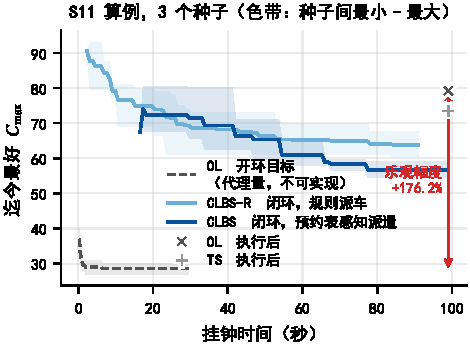
\includegraphics[width=\columnwidth]{fig/fig_convergence_closedloop_CN.pdf}
\Description{Best-so-far makespan against wall-clock time for the ladder
configurations, with the open-loop curve marked as a surrogate objective and its
realizable value shown as a separate point. Each curve carries a shaded band
giving the min-to-max range across the three seeds.}
\caption{单个 \texttt{funnel} 算例上的收敛曲线（示意，取自收敛诊断批次，见表~\ref{tab:batches}）。横轴为挂钟时间，曲线为三个种子的逐时刻均值，阴影带为种子间全距。
实线（B1、B2）为可实现的完工时间；虚线为开环搜索实际优化的代理目标；叉号与十字为同一计划经无冲突路由执行后的完工时间。
虚线终点与叉号之差即乐观幅度：开环并非收敛不充分，而是收敛到不可实现的代理目标。}
\label{fig:convergence}
%% 由 fig/fig_convergence_CN.py 生成(输出名 fig_convergence_closedloop_CN),
%% 数据源 clbs/output/ladder_convergence.csv 与 ladder_cost.csv,由 tools/ladder_diag.py 落盘。
%% 该图是说明性的:它画形状与落差,不承载统计主张,故只取三算例三种子,正文统计一律以
%% baseline_ladder.csv 为准。此口径已写在 ladder_diag.py 的首部注释里。
\end{figure}

\paragraph{预约表感知派遣是次要来源}
固定开环或闭环、只改变选车规则。闭环内 $\text{B1}\to\text{B2}$ 为 $-\GainProbeLoop$（$p\PProbeLoop$），伪中位数 \HLProbeLoop{}，$95\%$ 置信区间 \CIProbeLoop{}，下端离零不到一个百分点。这是合计结论：逐组校正后无一组显著（校正前 \CellsSigProbe{} 组），且车机比 $1.0$ 与 $2.0$ 两组上 B2 慢于 B1（表~\ref{tab:bytag}），因此不能逐组套用。
开环下 $\text{B0}\to\text{B0+}$ 为 $-\GainProbeOpen$（$p\PProbeOpen$），同样显著，但量级远小于闭环的 \GainLoopRule{}。

\paragraph{端到端效果与两项技术的关系}
\label{sec:complement}
$\text{B0}\to\text{B2}$ 合计为 $-\GainEndToEnd$（$p\PEndToEnd$，$\NPairs$ 个配对中 $\WinEndToEnd$ 胜 $\LoseEndToEnd$ 负 $1$ 平），即完工时间降低约五分之一。三个增益的比较基准不同，不能直接相加。若两项技术彼此独立，端到端增益应为 \GainLoopRule{} 与 \GainProbeOpen{} 的复合，即 \GainIndepProduct{}；实测 \GainEndToEnd{} 略低于此，说明二者各自起作用、彼此不放大。
由此也可解释「先排产、后解冲突」路线的不足：同一派遣规则放在两阶段结构中（B0+），收益只有 \GainProbeOpen{}；要获得闭环的降幅，让行等待必须在搜索时进入适应度。

\subsection{不同算例类别上的结果}
\label{sec:whichcongestion}

本节按布局、车机比与柔性三族拆开合计结果。三族各有一个预期：布局族检验收益是否随争用强度增长；车机比族检验是否存在 AGV 数量上界，超过后派遣收益被试算开销抵消；柔性族检验收益是否依赖改派余地。

\paragraph{单组的统计分辨率}
逐组检验按族做 Holm 校正，族取一个效应的 $\NCases$ 组（闭环与派遣各成一族）。闭环校正后仍有 \CellsSigLoopAdj{} 组显著（校正前 \CellsSigLoop{} 组，校正后最大 $p\PLoopCellMax$）；唯一例外是 AGV 最少的一组（\GainLoopStarve{}，不显著）。因此闭环的趋势可以按族解读。
派遣校正前有 \CellsSigProbe{} 组显著（柔性族两端，$p\PProbeFlexLoRaw$ 与 $p\PProbeFlexHiRaw$），校正后为 \CellsSigProbeAdj{} 组（Holm：$p\PProbeFlexLoHolm$ 与 $p\PProbeFlexHiHolm$；BH：$p\PProbeFlexLoBH$ 与 $p\PProbeFlexHiBH$）。其量级（数个百分点）与单组 $\NSeeds$ 个种子能分辨的下限同阶，因此下文对派遣只报告方向。

\begin{table}[t]
\caption{逐组的四级基线结果与闭环、派遣两个效应，按三族分块（每组 $n=\NSeeds$ 个按种子配对的比较）。
显著性标记按 \textbf{Holm 校正后}的 $p$ 给出（双侧 Wilcoxon 符号秩检验），族为一个效应的
$\NCases$ 组：$^{*}p<0.05$、$^{**}p<0.01$；$^{\dagger}$ 表示校正前显著、校正后不显著，该组符号不作结论。
负值表示完工时间下降。两个增益列与表~\ref{tab:main} 为同一估计量（逐对相对增益在种子上的均值），不能由同行两个均值相除得到。
\texttt{A funnel} 同时是 B 族 $N_A/N_M=1.5$ 与 C 族 $F=0.6$，只运行一次，只列一行。}
\label{tab:bytag}
\small
%% 由 tab/gen_tables_ladder.py 生成,按 A/B/C 三族分块。
%% 逐格增益列为"逐对相对增益的均值",与 tab_main 及导言区宏同源;显著性标记按 Holm 校正后的 p 值,
%% "校正前显著、校正后不显著"的格加印剑号。
%% 由 tab/gen_tables_ladder.py 生成,请勿手工编辑
%% 数据源:clbs/output/baseline_ladder.csv 等,见脚本首部
\begin{tabular}{@{}lrrrrrrrr@{}}
\toprule
& & \multicolumn{4}{c}{$C_{\max}$(时间单位)} & \multicolumn{3}{c}{本文相对对比方法的逐对相对差} \\
\cmidrule(lr){3-6}\cmidrule(lr){7-9}
算例 & 争用强度 & OL & TS & AE & \textbf{CLBS} & OL$\rightarrow$CLBS & TS$\rightarrow$CLBS & AE$\rightarrow$CLBS \\
\midrule
A S11 & 47.0\% & 77.25 & 68.90 & 84.65 & 54.75 & $-28.0\%^{*}$ & $-18.9\%^{*}$ & $-34.9\%^{*}$ \\
A S21 & 46.4\% & 68.50 & 63.35 & 80.55 & 51.95 & $-23.2\%^{*}$ & $-17.1\%^{*}$ & $-34.8\%^{*}$ \\
A S22 & 22.0\% & 61.55 & 55.20 & 70.35 & 45.50 & $-24.1\%^{*}$ & $-16.5\%^{*}$ & $-34.8\%^{*}$ \\
A GC & 19.4\% & 90.90 & 80.70 & 94.85 & 67.40 & $-24.3\%^{*}$ & $-15.5\%^{*}$ & $-28.4\%^{*}$ \\
A GD & 16.2\% & 93.10 & 82.95 & 92.60 & 66.50 & $-28.1\%^{*}$ & $-19.5\%^{*}$ & $-27.7\%^{*}$ \\
\midrule
B $N_A/N_M=0.5$ & 27.3\% & 130.45 & 131.50 & 130.30 & 113.55 & $-12.4\%^{*}$ & $-12.8\%^{*}$ & $-12.1\%^{*}$ \\
B $N_A/N_M=1.0$ & 49.4\% & 96.10 & 97.80 & 101.50 & 80.05 & $-15.3\%^{*}$ & $-17.1\%^{*}$ & $-20.6\%^{*}$ \\
B $N_A/N_M=2.0$ & 47.2\% & 72.65 & 61.65 & 82.10 & 61.65 & $-14.5\%^{*}$ & $+0.2\%$ & $-24.6\%^{*}$ \\
\midrule
C $F=0.3$ & 47.3\% & 90.90 & 77.00 & 101.80 & 63.00 & $-30.3\%^{*}$ & $-17.6\%^{*}$ & $-38.0\%^{*}$ \\
C $F=1.0$ & 49.0\% & 75.60 & 69.30 & 89.10 & 57.25 & $-22.0\%^{*}$ & $-15.4\%^{\dagger}$ & $-35.5\%^{*}$ \\
\bottomrule
\end{tabular}

\end{table}

\begin{figure}[t]
\centering
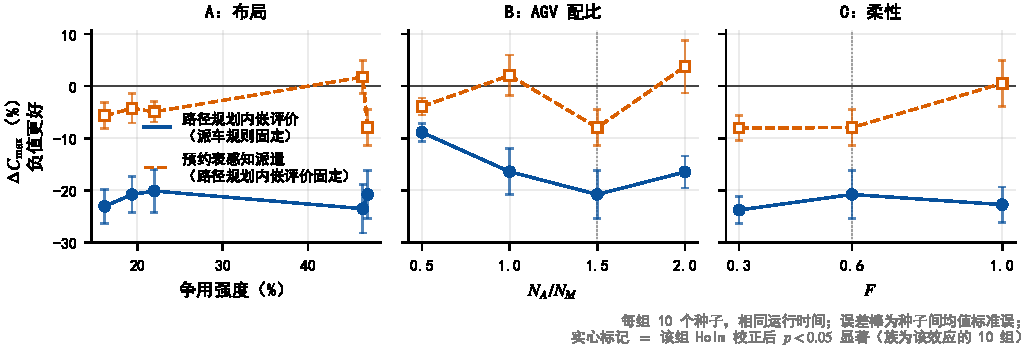
\includegraphics[width=\columnwidth]{fig/fig_prediction3_CN.pdf}
\Description{Three panels of line plots: closed-loop gain and reservation-aware
dispatch gain across layout (vs contention), fleet-to-machine ratio, and flexibility. After
Holm correction over the ten cells the closed-loop curve is filled, hence
significant, at nine of ten cells, while the dispatch curve is hollow at every
cell, and its sign alternates across the four fleet-ratio levels. Error bars
give the standard error of the mean over the ten seeds of each cell; the
dispatch bars cross zero at every cell and the closed-loop bars do not.}
\caption{闭环与派遣增益在三族上的分布。左：布局族，横轴为争用强度；中：车机比 $N_A/N_M$；右：柔性。
B、C 两族含共用基点（空心竖线处的 $1.5$ 与 $0.6$）。
实心为 Holm 校正后仍显著（$p<0.05$），空心为不显著；误差棒为 $\NSeeds$ 个种子上的均值标准误。
闭环 \CellsSigLoopAdj{} 组显著，大体随争用上升；派遣校正后无一组显著，误差棒逐组跨零。}
\label{fig:prediction3}
%% 由 fig/fig_prediction3_CN.py 从 clbs/output/baseline_ladder.csv 生成。横轴:A 族取争用强度,
%% B/C 族取算例名末尾的因子水平;基点 A funnel 的 (1.5, 0.6) 由脚本按 abc_matrix.BASE 显式补入。
%% 填充判据为 Holm 校正后的 p 值,族取该效应的全部十格。
\end{figure}

\paragraph{布局族}
闭环五组均显著，且大体随争用上升：最不拥堵的 \texttt{scatter}（争用 \ContentionLo{}）为 \GainLoopScatter{}，\texttt{mid}/\texttt{low} 为 \GainLoopMid{}/\GainLoopLow{}，\texttt{funnel}/\texttt{high} 为 \GainLoopFunnel{}/\GainLoopHigh{}。
有两处逆序。\texttt{low} 争用高于 \texttt{mid} 而收益更小，但二者跨越脊式与网格的拓扑分界，最远行程也不同（\LegGrid{} 对 \LegDumbbell{}）。\texttt{funnel} 争用高于 \texttt{high} 而收益更小，二者是只差一条出口的单因素对照，构成真正的反例。
因此可以确定的是量级（最拥堵一组约为最不拥堵一组的两倍半），而非争用与收益的单调关系；争用强度把拥堵概括为一个数，不区分其中可由改派绕开的部分（第~\ref{sec:limitations}~节局限 (1)）。派遣五组中四组为负，与闭环同向。

\paragraph{车机比族}
闭环内派遣在 $N_A/N_M=0.5$、$1.0$、$1.5$（基点）、$2.0$ 上依次为 $-\GainProbeStarve$、\GainProbeFleetOne{}、\GainProbeFleetBase{}、\GainProbeFleetTwo{}，符号交替，四组均不显著（校正前 $p\PProbeFleetHalfRaw$、$p\PProbeFleetOneRaw$、$p\PProbeFleetBaseRaw$、$p\PProbeFleetTwoRaw$）。若只看 $0.5$、$1.0$、$2.0$，曲线呈现第~\ref{sec:costlaw}~节开销规律所预测的上升；计入基点后这一趋势不再成立。因此本族未能确定派遣收益的 AGV 数量上界，检验它需要足以分辨数个百分点效应的种子数。闭环在 $1.0$ 与 $2.0$ 上为 \GainLoopFleetOne{} 与 \GainLoopFleetTwo{}，均显著。

\paragraph{柔性族}
派遣在 $F=0.3$、$0.6$、$1.0$ 上为 \GainProbeFlexLo{}、\GainProbeFleetBase{} 与 \GainProbeFlexHi{}，三者同号，两端是全部 $\NCases$ 组中量级最大的两组，但校正后（$p\PProbeFlexLoHolm$、$p\PProbeFlexHiHolm$）不显著。若派遣依赖改派余地，$F=0.3$ 应最先失效，而该组恰是量级最大的一组；这与「派遣主要通过选车与时序调整起作用」相容。闭环为 \GainLoopFlexLo{} 与 \GainLoopFlexHi{}，逐组显著。

\paragraph{独立算例上的交叉核对}
另用一批算例核心与基线都不同的自建算例核对：$\MatrixCells$ 组 $\times$ $10$ 种子，共 $\MatrixRuns$ 次运行，基线为两阶段代理运输，在四个争用水平与四个异构度水平上交叉。集成增益（两阶段 $\to$ 闭环）为 \GainIntegMatrix{}，$\MatrixCells$ 组中 \SigIntegMatrix{} 组显著（未校正），区间 \GainIntegMatrixLo{} 到 \GainIntegMatrixHi{}，与本节闭环的方向和量级一致。

\paragraph{异构度没有抬高闭环收益}
该批按 $H$ 分为四个水平（每个水平 $4$ 组）：$H=0$ 为 \GainIntegHZero{}，$H=0.15$（实测 \MatrixHMeasLow{}）为 \GainIntegHLow{}，$H=0.3$ 为 \GainIntegHMid{}，$H=0.5$ 为 \GainIntegHHigh{}；增益与 $H$ 的秩相关为 \RhoIntegH{}。实测 $H=\MatrixHMeasLow$ 接近公开算例中位 \PubHMed{}，其增益与 $H=0.3$ 相差不到半个百分点，因此把 $H$ 定在文献区间之上并未抬高闭环收益。每个水平只有 $4$ 组、组内散布远大于水平间差距，故只支持「收益不随 $H$ 上升」。
这与第~\ref{sec:features}~节的分析相符：$H$ 增大时，指派越来越多由加工速度而非通行条件决定。$H=0$ 时改派不必用加工时间换通行时间，成为代价为零的避堵决策，该水平增益最高（\GainIntegHZero{}）。$H$ 使机器选择成为权衡（没有异构，第~\ref{sec:Chapter_I}~节的反转不会出现），但闭环收益来自搜索时是否计入让行，争用强弱由布局与 AGV 数量决定。
该批对预约表感知派遣给出 \GainProbePre{}（$0$ 组显著），与主批次方向相反；该批运行于两项加速之前，原因见第~\ref{sec:costlaw}~节。

\subsection{计算开销与两项加速}
\label{sec:costlaw}

在固定挂钟预算下，单次评价开销与可完成的评价次数此消彼长。同一派遣规则在加速前净效果不显著、加速后显著为正，故本节直接度量二者。

\paragraph{两种预算口径}
图~\ref{fig:protocol} 给出各配置的单次评价开销与同一预算内完成的评价次数：开销跨越约两个数量级，开环仅用约两成挂钟即完成了最多的评价次数。
图~\ref{fig:protocols} 把同一组比较在两种口径下各做一次。同代数口径不计额外开销，偏向开销高的配置：预约表感知派遣相对规则派车为 \GainProbeSameGen{}（$p\PProbeSameGen$）；同挂钟下、加速之前仅为 \GainProbeSameClock{}（$p\PProbeSameClock$），接近零。前者回答额外的路由计算是否改进了每一代的排序，后者回答相同时间内完工时间是否下降，二者不能相互替代。

\begin{figure}[t]
\centering
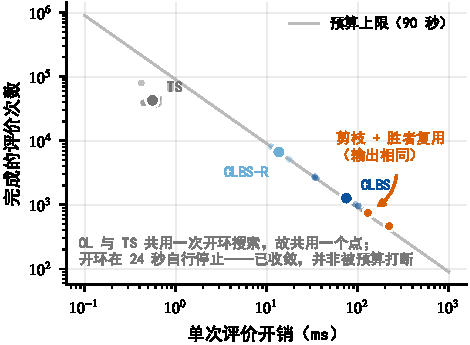
\includegraphics[width=\columnwidth]{fig/fig_protocol_CN.pdf}
\Description{A log-log scatter of cost per evaluation against evaluations
completed. A grey hyperbola marks the 90-second budget cap. The two closed-loop
configurations sit on it, while the open-loop configuration sits well below it
because it stalls after about seventeen seconds. Orange markers are the
pruning ablation off and on; a callout marks the on setting.}
\caption{单次评价开销与完成的评价次数。灰线为 $90$ 秒预算上限，点落在线上表示开销 $\times$ 次数等于该配置的挂钟。两个闭环配置落在线上，即每次都用满预算；开环落在线下方，因其约 $17$ 秒即由早停终止，并非被预算截断。
B0 与 B0$^+$ 共用同一次开环搜索，故共用一个点。淡色小点为三个算例的逐个测量值，实心大点为其几何平均。
橙色圆点为两项加速的关闭与开启（引出线标出开启者）；由命题~\ref{prop:speedup_equiv}，二者输出相同，沿该线的位移仅反映算力节省。}
\label{fig:protocol}
%% 由 fig/fig_protocol_CN.py 生成(输出名 fig_protocol_CN),数据源 clbs/output/ladder_cost.csv
%% 与 prune_ablation.csv;后者缺失时脚本自动省略橙色圆点而不报错。
\end{figure}

\begin{figure}[t]
\centering
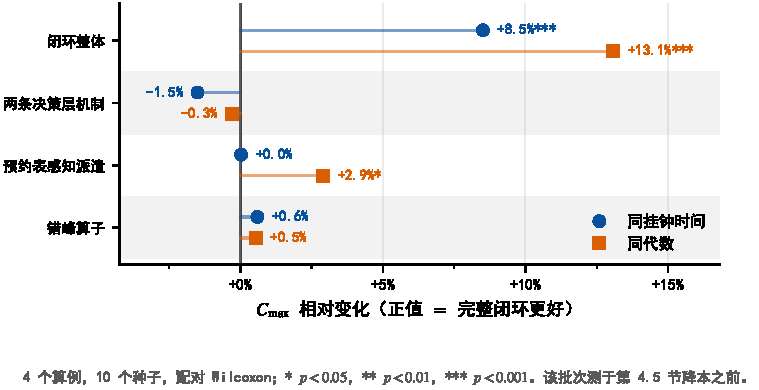
\includegraphics[width=\columnwidth]{fig/fig_protocols_CN.pdf}
\Description{The same paired comparisons shown twice, once under an equal
wall-clock budget and once under an equal number of generations.}
\caption{同一组比较在两种预算口径下的结果，每一行按其所隔离的机制命名。
预约表感知派遣在同代数下为 \GainProbeSameGen{}（$p\PProbeSameGen$），同挂钟下为 \GainProbeSameClock{}（$p\PProbeSameClock$）。
该批运行于两项加速之前（表~\ref{tab:batches}）。}
\label{fig:protocols}
%% 由 fig/fig_protocols_CN.py 从 clbs/experiments/protocols.csv 生成(4 算例 x 10 种子)。
\end{figure}

\paragraph{开销规律}
预约表感知派遣把每个运输任务的路由调用从 $2$ 次增至至多 $2N_A$ 次，开销随 AGV 数量线性增长。剪枝所用下界在争用越弱时越紧，跳过的候选越多。实测与此一致：六组中路由调用削减率最高的是最不拥堵的一组（\RouteCallCutHi{}），最低的是 AGV 最多的一组（\RouteCallCutLo{}），剪枝效果减弱但未失效。二者合起来\emph{预测}：AGV 足够多、争用足够强时，试算开销将抵消派遣收益。第~\ref{sec:whichcongestion}~节车机比族未能证实这一上界；开销规律本身是直接测得的，由它推出的上界尚未验证。

\paragraph{单独开关两项加速}
为排除批次差异，另做一组只改变加速开关的对照：同算例、同种子、同预算。先做等价性自检：六个算例上各取六条随机染色体，开启与关闭加速时的完工时间与派车序列\emph{逐位相同}，$36$ 组无一例外，与命题~\ref{prop:speedup_equiv} 一致；路由调用合计减少 \RouteCallCut{}。因此同挂钟下的完工时间差\emph{仅}来自节省的算力。
结果见表~\ref{tab:prune}：开启加速使完工时间再降 \GainPrune{}（\WinPrune{} 胜 / \LosePrune{} 负，$p\PPrune$），同预算内评价次数为 \EvalRatioPrune{} 倍，单次评价加速 \SpeedupProbe{} 倍。这一对照衔接了两个批次：同一派遣规则在加速前的独立批次上为 \GainProbePre{}（$0$ 组显著），加速后在主批次上显著为正。

\begin{table}[t]
\caption{只改变两项加速（下界剪枝与胜者路径复用）。「关」/「开」指二者是否启用，加粗表头为本文采用的设置。
两种设置输出逐位相同，差值仅来自节省的算力。同算例、同种子、同挂钟；$n=60$ 配对，双侧 Wilcoxon 符号秩检验（$^{***}p<0.001$）。
两个比值列的分母都是\emph{关}的值：评价次数按 开/关，单次评价耗时按 关/开。}
\label{tab:prune}
\small
%% 数字与 clbs/output/prune_ablation.csv / 运行日志一致;亦可用
%% py paper01/tab/gen_tables_ladder.py 从同一 CSV 重生成。
%% 由 tab/gen_tables_ladder.py 生成,请勿手工编辑
%% 数据源:clbs/output/baseline_ladder.csv 等,见脚本首部
\begin{tabular}{@{}lrrrrrr@{}}
\toprule
& & \multicolumn{2}{c}{$C_{\max}$(时间单位)} & & 评价次数比 & 单次评价加速比 \\
\cmidrule(lr){3-4}
算例 & 争用强度 & 关 & \textbf{开} & $\Delta C_{\max}$ & (开/关) & (关/开) \\
\midrule
\texttt{S11} & 47.0\% & 64.50 & 58.40 & $-9.46\%$ & 2.11$\times$ & 2.20$\times$ \\
\texttt{S21} & 46.4\% & 57.30 & 52.50 & $-8.38\%$ & 2.19$\times$ & 2.37$\times$ \\
\texttt{GC} & 19.4\% & 73.90 & 70.90 & $-4.06\%$ & 2.88$\times$ & 3.37$\times$ \\
$N_A/N_M=0.5$ & 27.3\% & 130.25 & 115.75 & $-11.13\%$ & 2.76$\times$ & 2.81$\times$ \\
$N_A/N_M=1.0$ & 49.4\% & 88.55 & 83.95 & $-5.19\%$ & 2.36$\times$ & 2.42$\times$ \\
$N_A/N_M=2.0$ & 47.2\% & 64.75 & 63.65 & $-1.70\%$ & 1.48$\times$ & 1.82$\times$ \\
\midrule
\emph{配对合计}(60 配对) & --- & --- & --- & $-6.48\%^{***}$ & \multicolumn{2}{r}{44/0/16,\ $<10^{-4}$} \\
\midrule
\multicolumn{7}{@{}l@{}}{\footnotesize HL 伪中位数与 $95\%$ CI:$-6.10$ $[-7.80,-4.51]$\,\%} \\
\bottomrule
\end{tabular}

\end{table}

\subsection{其他层间接口的对照}
\label{sec:pricing}

本节报告第~\ref{sec:interface}~节两种接口的结果。主批次中附加代价关闭（$\theta=0$）；按让行记录的局部搜索在四个配置中以相同设置启用，不影响配置之间的比较。

\paragraph{按让行记录的局部搜索}
在第~\ref{sec:whichcongestion}~节的 $\MatrixCells$ 组独立数据中，关掉让行记录的相对增益为 \GainCertMatrix{}（仅 $1$ 组显著），关掉错峰算子为 \GainStaggerMatrix{}（$2$ 组显著），均不为正：在相同挂钟下，把解码次数用于该邻域，不如用于种群进化。让行记录与错峰在两项加速前后没有改动，开销也不随剪枝变化，故可引用该批较早的数据；派遣则不行，因为其开销正是加速的对象。

\paragraph{走廊时段附加代价}
第~\ref{sec:interface}~节指出，附加代价会重复计入适应度已含的延误，但这一论证不能给出完工时间变差的幅度，故单独度量。实验在两种预算口径下扫描 $\theta$，并在所有 $\theta$ 上固定路径搜索的宽度。

\begin{figure}[t]
\centering
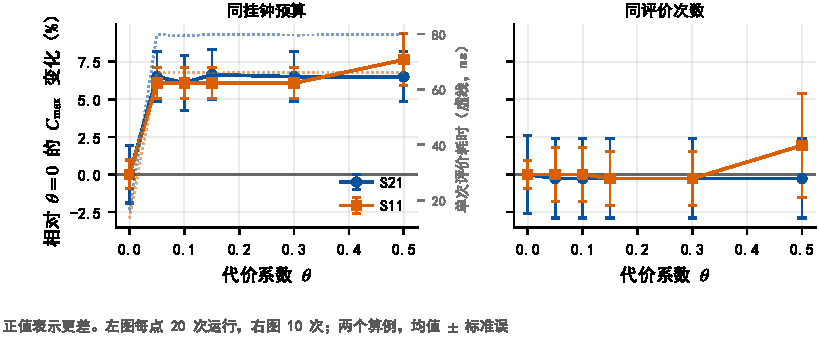
\includegraphics[width=\columnwidth]{fig/fig_theta_CN.pdf}
\Description{Two panels of makespan change relative to theta equals zero against
pricing strength: under equal wall-clock the penalty is large and flat, under
equal evaluations it is absent. Markers are means over seeds and error bars are
the standard error of the mean. The batch is two separately generated instances
that are not members of the paper's A/B/C families.}
\caption{走廊时段附加代价的影响，正值表示更差。同挂钟（左）下，完工时间变差在附加代价一开启即出现，并在 $\theta$ 的十倍范围内平坦，与右轴的单次评价开销同步；同评价次数（右）下变差消失。
标记为均值，误差棒为均值标准误；「显著」指每个 $\theta$ 与 $\theta=0$ 按种子配对的双侧 Wilcoxon 检验。
两个算例不属于表~\ref{tab:instances} 的三族，批次见表~\ref{tab:batches}。}
\label{fig:theta}
%% 由 fig/fig_theta_CN.py 从 clbs/experiments/theta_sweep.csv 与 theta_sweep_gen.csv 生成
%% (08-05 落盘,2 算例 x 10 种子,左图每点 20 次运行、右图 10 次)。
%% 该批次属加速之前的测量;附加代价机制在加速前后未改动,且其开销与剪枝无关,故该测量对它依然有效。
\end{figure}

如图~\ref{fig:theta} 所示，同挂钟下每个 $\theta$ 都使完工时间显著变差，且在十倍范围内平坦；同评价次数下不显著。带附加代价的路由在同一预算内完成的评价次数约为不带时的五分之一，即损害来自评价次数减少，而非候选解排序出错。
另有两点可排除其他解释。其一，在两个数量级的 $\theta$ 范围内，带附加代价的路由修改的是相同的少数路径，累计附加代价只占总行驶时间的很小一部分，不足以改变到达时刻的次序；只有 $\theta$ 大到附加代价超过到达时刻时，重复计入的影响才显现。其二，开销是结构性的：有无附加代价的耗时之比在每个 $\theta$ 上都相同，额外开销来自多标签 Pareto 搜索本身，与引理~\ref{lem:label} 一致。
因此，只要适应度取自完整的无冲突解码，附加代价就不含新信息，结果由其额外开销决定。扩充层间接口之前，应先检查接收层的目标是否已包含该接口要传递的量。

\subsubsection{失效原因：稀释与开销}
\label{sec:whycost}

\paragraph{解码次数的分配}
按让行记录的局部搜索消耗了很大一部分解码次数，而所解码的邻居中能改进完工时间的不到五十分之一。该邻域规模小且指向明确（第~\ref{sec:ls}~节），命中率仍低，说明记录所指的工序在改派或错峰后并不能缩短关键链。本文另试了三种改进：按预期让行而非畅通时间为改派打分、把错峰改为定向插入、接受完工时间不变但总让行下降的平台移动；在同评价次数下均不显著。因此失效源于信号本身，而非其使用方式。

\paragraph{沿关键链的稀释}
一份让行记录指明的是消除\emph{一次}让行所需的信息。完工时间由一条链决定，消除一处走廊延误后，另一约束（上游工序、某台机器或另一条走廊）通常随之成为紧约束，实际改进只是被消除延误的一部分。当一个瓶颈只是若干量级相当的瓶颈之一时，针对它的改进远小于被消除的让行时长。

\paragraph{派遣在加速前后结果不同的原因}
同样的稀释也作用于预约表感知派遣：试算选出的是当前任务送达最早的 AGV，这一局部改进传到完工时间时只保留一部分，降幅仍为正，但只有数个百分点。加速之前，单次评价开销为规则派车的 \CostMultBefore{} 倍，同一挂钟内评价次数不足，净效果不显著；开销降至 \CostMultAfter{} 倍之后，降幅才在合计上显著。
因此两种机制的失效原因不同：按让行记录的局部搜索受限于稀释后剩余的降幅过小；派遣受限于单次评价开销，而这一开销可以在不改变结果的前提下降低。本文因此把派遣列为方法贡献，把按让行记录的局部搜索只作为受控负对照报告。

\subsection{案例分析}
\label{sec:casestudy}

本节在单个漏斗算例上并列 B0 与 B2，说明一次求解中发生了什么。图~\ref{fig:case_gantt} 把加工机器与 AGV 画在同一时间轴上。可见三点：开环解中，让行成段出现在上下料点附近的走廊上，并集中于少数几辆 AGV；闭环解大幅减少了这些等待，且若干道工序被指派到并非最快的机器，即以较长加工换取更通畅的路径（式~\eqref{eq:reassign}）；闭环解的 AGV 负载也更均衡，这是前两点的结果。

\begin{figure*}[t]
\centering
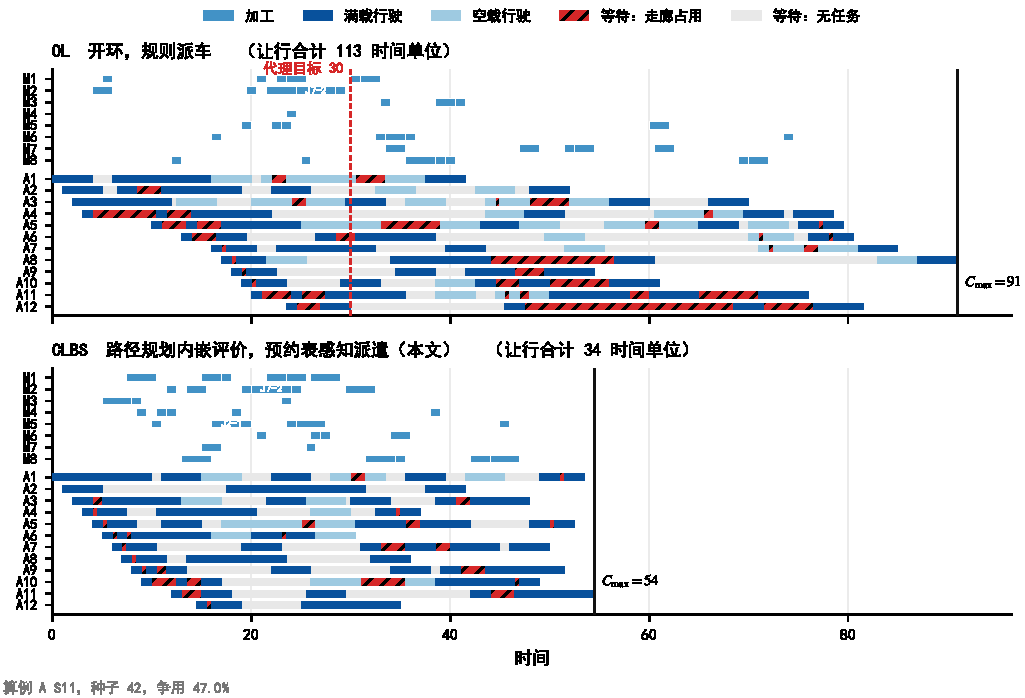
\includegraphics[width=\textwidth]{fig/fig_case_gantt_CN.pdf}
\Description{Side-by-side Gantt charts of the open-loop and closed-loop
solutions on one funnel instance, with machines and vehicles on a shared time axis
and yielding waits shaded separately.}
\caption{同一漏斗算例上 B0（上）与 B2（下）的甘特图。加工机器与 AGV 共用时间轴；AGV 行区分空载、满载与两类空隙：同一运输任务两段之间的空隙为让行等待，不同任务之间的空隙为 AGV 空闲，二者以不同颜色区分。}
\label{fig:case_gantt}
%% 由 fig/fig_case_gantt_CN.py 从 clbs/output/case_study/*.json 生成(tools/ladder_diag.py
%% 的 --case-study 落盘)。让行/空闲的区分由脚本从相邻段的 task 字段推出,不是另存的标注。
\end{figure*}

图~\ref{fig:case_chain} 按表~\ref{tab:attrib} 给关键链各节着色。B0 的链上 \texttt{corridor} 占显著比例；B2 上它们大体消失，取而代之的是 \texttt{machine} 与 \texttt{upstream}。这正是第~\ref{sec:whycost}~节所述的稀释：消除一处走廊延误后，另一约束成为紧约束。

\begin{figure}[t]
\centering
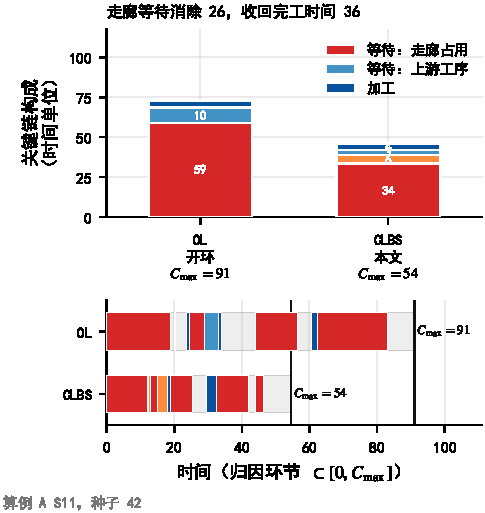
\includegraphics[width=\columnwidth]{fig/fig_case_chain_CN.pdf}
\Description{The critical chain of the open-loop and closed-loop solutions,
with each link coloured by its attribution label.}
\caption{关键链各节按表~\ref{tab:attrib} 着色。上：B0 与 B2 关键链的构成，标题并列「被消除的走廊等待」与「实际缩短的完工时间」，二者之差即被新的紧约束吸收的部分。下：同一条链在时间轴上的位置。}
\label{fig:case_chain}
%% 由 fig/fig_case_chain_CN.py 从同一批 case_study/*.json 生成;归因标签直接取
%% algorithm/decoder.py 的 critical_chain(),五类标签一个不并、不归入 other。
\end{figure}

\subsection{公开基准上的上层搜索标定}
\label{sec:external}

前文各节比较的是同一实现的不同配置，配置之间的差值不受实现水平影响，但无法说明上层搜索本身的强弱。本节用公开基准标定上层搜索。

\paragraph{比较设定}
删去走廊排他约束式~\eqref{eq:excl} 后，本文模型精确退化为标准 FJSP\_PT（第~\ref{sec:fjsppt}~节），与公开基准是同一个数学问题；另取 $\delta_{\mathrm{ret}}=0$，以对齐其完工时间定义。退化后没有走廊争用，两项技术都不起作用，检验的只是上层搜索。
算例取 Homayouni 与 Fontes~\cite{homayouni2021production} 整理的 \PubNInst{} 个算例（源自 Fattahi 等~\cite{fattahi2007mathematical}，$2$--$12$ 个工件、$4$--$48$ 道工序、$2$--$8$ 台机器），按 Lim 与 Moon~\cite{lim2023twophase} 的设定取两辆 AGV、成品不回运。运输时间原样采用所发布的矩阵，直接作为 $t^{*}$，不做最短路合成（其中 \PubNLayoutBad{} 个矩阵不是任何图的最短路闭包，合成会改变算例）。两个小型算例（\textsc{sfjst}01、\textsc{sfjst}03）的文献最优值已手算核对，确认均不含回运。参照值中，\PubNOpt{} 个算例有 MILP 证明的最优值~\cite{homayouni2021production}，其余 $4$ 个取已发表最好值~\cite{lim2023twophase}。

\paragraph{结果}
表~\ref{tab:external} 为 \PubNInst{} 个算例 $\times$ \NSeeds{} 个种子。全部 $200$ 次运行均通过校验，没有低于复合下界的解；在有可证最优值的 \PubNOpt{} 个算例（$160$ 次运行）上，没有任何一次低于最优值，这验证了模型转换的正确性。
$\PubNMatch{}/\PubNInst{}$ 个算例的最优解与参照值逐位相同，其中 $10$ 个小型算例（\textsc{sfjst}01--10）全部命中；平均间隙 \PubGapMean{}（中位 \PubGapMed{}）。间隙大体随规模上升：四个最大算例（$32$--$48$ 道工序）均值为 \PubGapBig{}、最差 \PubGapMax{}；不超过 $24$ 道工序的 $16$ 个算例无一超过 $5.45\%$。

\begin{table}[t]
\caption{公开基准上的退化比较（删去排他约束，与文献同一问题）。「参照」列的
\textsc{opt} 为 MILP 证明的最优值、\textsc{bk} 为已发表最好值；间隙以 \NSeeds{} 个种子的最优
解计。星号标出最优解与参照值逐位相同者。}
\label{tab:external}
\centering
\small
%% 由 tab/gen_tables_ladder.py 生成,请勿手工编辑
%% 数据源:clbs/experiments_database/gap_ideal.csv;工序数取自 clbs/database/json/hf/*.json
\begin{tabular}{lrrrrrr}
\toprule
& & & \multicolumn{3}{c}{$C_{\max}$(时间单位)} & \\
\cmidrule(lr){4-6}
算例 & 工序 & 参照 & \multicolumn{1}{c}{值} & 最优 & 均值 & 间隙 \\
\midrule
SFJST01 & 4 & \textsc{opt} & 70 & 70\rlap{$^*$} & 70.0 & 0.00\% \\
SFJST02 & 4 & \textsc{opt} & 111 & 111\rlap{$^*$} & 111.0 & 0.00\% \\
SFJST03 & 6 & \textsc{opt} & 223 & 223\rlap{$^*$} & 223.0 & 0.00\% \\
SFJST04 & 6 & \textsc{opt} & 359 & 359\rlap{$^*$} & 359.0 & 0.00\% \\
SFJST05 & 6 & \textsc{opt} & 123 & 123\rlap{$^*$} & 123.0 & 0.00\% \\
SFJST06 & 9 & \textsc{opt} & 324 & 324\rlap{$^*$} & 324.0 & 0.00\% \\
SFJST07 & 9 & \textsc{opt} & 409 & 409\rlap{$^*$} & 409.0 & 0.00\% \\
SFJST08 & 9 & \textsc{opt} & 269 & 269\rlap{$^*$} & 269.5 & 0.00\% \\
SFJST09 & 9 & \textsc{opt} & 220 & 220\rlap{$^*$} & 222.0 & 0.00\% \\
SFJST10 & 12 & \textsc{opt} & 531 & 531\rlap{$^*$} & 531.0 & 0.00\% \\
MFJST01 & 15 & \textsc{opt} & 485 & 485\rlap{$^*$} & 485.0 & 0.00\% \\
MFJST02 & 15 & \textsc{opt} & 463 & 476 & 483.4 & 2.81\% \\
MFJST03 & 18 & \textsc{opt} & 482 & 482\rlap{$^*$} & 504.7 & 0.00\% \\
MFJST04 & 21 & \textsc{opt} & 576 & 586 & 623.0 & 1.74\% \\
MFJST05 & 21 & \textsc{opt} & 532 & 561 & 592.8 & 5.45\% \\
MFJST06 & 24 & \textsc{opt} & 652 & 677 & 728.3 & 3.83\% \\
MFJST07 & 32 & \textsc{bk} & 898 & 965 & 1023.3 & 7.46\% \\
MFJST08 & 36 & \textsc{bk} & 900 & 970 & 1027.0 & 7.78\% \\
MFJST09 & 44 & \textsc{bk} & 1098 & 1226 & 1279.2 & 11.66\% \\
MFJST10 & 48 & \textsc{bk} & 1230 & 1389 & 1473.0 & 12.93\% \\
\bottomrule
\end{tabular}

\end{table}
%% 由 tab/gen_tables_ladder.py 的 tab_external() 从
%% clbs/experiments_database/gap_ideal.csv 生成;"工序"列由脚本从 clbs/database/json/hf/*.json 现数,不得手填。
%% 同一函数还打印 \PubNInst、\PubNOpt、\PubNMatch、\PubGapMean、\PubGapMed、
%% \PubGapMax、\PubGapBig、\PubGapMeanSeed、\PubLBSlack、\PubLBTotal 十个导言区宏。

\paragraph{间隙主要源于搜索能力}
文献中最大算例的 MILP 耗时近十小时（\textsc{mfjst}06，$34\,796$ 秒），本文每次运行只用数秒。在间隙集中的 $10$ 个 \textsc{mfjst} 算例上提高预算（代数上限五倍、早停阈值 $3.3$ 倍，实测挂钟为 \PubBudgetRatio{} 倍）重跑，平均间隙仅从 \PubGapLoBudget{} 降到 \PubGapHiBudget{}（$\PubBudgetGainPP$ 个百分点），其中 \PubBudgetNoGain{} 个未见下降。两种预算下全部 $300$ 次运行均由早停终止，未触及代数上限。因此间隙主要反映上层搜索的能力边界，而非预算不足（改进方向见第~\ref{sec:future_work}~节第 (3) 条）。

\paragraph{下界间隙的来源}
自建算例上复合下界与最好解的间隙中位数为 \LBGapMed{}，它包含下界的松弛与搜索的不足两部分，在最优值未知时无法区分。在 \PubNOpt{} 个有可证最优值的公开算例上可以区分：同一复合下界比最优值低出的中位数为 \PubLBSlack{}，比本文最好解低出的中位数为 \PubLBTotal{}；搜索解高出最优的中位数为 $\PubLBResidMed$ 个百分点，最大为 $\PubLBResidMax$ 个百分点。可见在无争用算例上，该间隙几乎全部来自下界的松弛。自建算例不能直接套用这一比例（下界不含争用，真实最优只会因争用而升高），但至少说明 \LBGapMed{} 不能解读为搜索差距；有争用时搜索与最优的距离仍未知（第~\ref{sec:limitations}~节局限 (3)）。



\section{结论}
\label{sec:Chapter_VI}

\subsection{工作总结}

本文研究机器指派与 AGV 无冲突路由须同时决策的柔性作业车间调度问题，聚焦运输耗时超过加工、拥堵集中于少数共享走廊的车间。在这类车间中，通往快速机器的走廊拥堵时，较慢但通行顺畅的机器可能是更优的选择，而常数运输时间模型看不到这一点。
为此，本文提出闭环双层框架：上层以文化基因算法搜索机器指派与工序顺序，下层以时间窗 Dijkstra 在走廊预约表上规划无冲突路径；通过路由内嵌评价与预约表感知派遣两项技术让路由结果进入排产，并以两项可证明不改变结果的加速降低派遣开销。实验以只改变一项机制的四级基线，在相同挂钟时间预算下分别度量了两项技术的收益与代价。

\subsection{主要结论}
\label{sec:contributions}

\textbf{(1) 路由内嵌评价是收益的主要来源。}
相对开环，闭环在规则派车下使完工时间降低 $\GainLoopRule$（$p\PLoopRule$），在预约表感知派遣下降低 $\GainLoopProbe$（$p\PLoopProbe$）；$\NCases$ 组中有 \CellsSigLoopAdj{} 组经 Holm 校正后仍显著。收益随争用强度大体上升，最拥堵一组约为最不拥堵一组的两倍半，但并非单调关系（第~\ref{sec:whichcongestion}~节）。

\textbf{(2) 预约表感知派遣是次要来源，其净收益依赖两项加速。}
闭环内派遣使完工时间再降低 $\GainProbeLoop$（$p\PProbeLoop$，$95\%$ 区间 \CIProbeLoop{}），开环下为 $\GainProbeOpen$（$p\PProbeOpen$），都只在合并各组检验时显著。两项加速不改变所选 AGV 与时间表（命题~\ref{prop:speedup_equiv}，并经逐位自检），使路由调用减少 \RouteCallCut{}、开销倍数由 \CostMultBefore{} 降至 \CostMultAfter{}，这是派遣在相同挂钟下取得净收益的前提。

\textbf{(3) 两项技术不能互相替代，也不相互放大。}
端到端降低 $\GainEndToEnd$，略低于独立复合的预测值 $\GainIndepProduct$。「先排产、后解冲突」的路线即使改用预约表感知派遣，也只能获得 $\GainProbeOpen$，拿不到闭环带来的 $\GainLoopProbe$（$\text{B0+}\to\text{B2}$）。

\subsection{局限}
\label{sec:limitations}

\textbf{(1) 算例族的范围。}
主实验固定规模、只改变结构，故不就机制随规模的变化作结论；$H$ 固定为 $0.3$，其影响只在规模较小的独立算例上检验过。布局族中只有三组脊式算例之间的差异可单独归因于容量，网格算例还同时改变了拓扑与距离（最远行程由 \LegDumbbell{} 升至 \LegGrid{}）；争用强度只用一个数概括拥堵，不区分可由改派绕开的部分。这两点可能是收益只「大体」随争用上升的原因。采用自建算例，是因为这一方向尚无带显式路网的公开基准（第~\ref{sec:instances}~节）。

\textbf{(2) 派遣收益只在合计上显著。}
其量级只有数个百分点，与种子间离散度同阶，在哪类算例上稳定出现尚不能确定（第~\ref{sec:whichcongestion}~节）。

\textbf{(3) 有走廊争用时，解与最优的距离未知。}
上层搜索已在无争用的公开基准上标定（第~\ref{sec:external}~节），但有争用的算例尚无可证最优值。这不影响配置之间的差值，但数个百分点量级的效应（如派遣的 \GainProbeLoop{}）可能与这一距离相当。

\textbf{(4) 附加代价与按让行记录的局部搜索未降低完工时间。}
二者都在同一实现、同一挂钟下判定。所有配置同比例加速时结论不变；只有单独降低某一接口的开销才可能改变结论（派遣的加速即为一例），届时须重新度量。

\textbf{(5) 未考虑故障与动态到达。}
结果限于工件与工时已知、设备不发生故障的静态设定（假设 A7）。出现故障或在线到达时，机制的价值还包括修复排程的速度，本文未度量。

\textbf{(6) 未测试运输不超过加工的车间。}
本文算例的 $\bar{T}_t/\bar{T}_p$ 标定为 $4.0$。运输不超过加工时，AGV 争用依然存在，但通常不是瓶颈，闭环收益预期较小。

\subsection{未来工作}
\label{sec:future_work}

\textbf{(1) 更大规模与更细的拥堵刻画。} 对应局限 (1)：在更大的显式走廊网络上检验收益是否保持同一量级；把「拥堵能否通过改派绕开」与「关键链上是否只有一个主导瓶颈」作为两个独立维度设计算例，并构造能区分前者的新指标。

\textbf{(2) 更多种子。} 对应局限 (2)：把种子数提高约一个数量级、车机比取更密的水平，确定派遣收益稳定出现的算例类别，并检验第~\ref{sec:costlaw}~节预测的 AGV 数量上界。

\textbf{(3) 有争用时的最优间隙。} 对应局限 (3)：小规模算例可用 van Os 与 Basten~\cite{vanos2026exact} 的精确方法求解；大规模算例上间隙对延长搜索不敏感，需要改进编码或邻域。

\textbf{(4) 增量评价。} 对应局限 (4)：解码器状态单向推进，扰动只作用于序列某一位置之后时，此前的事件与预约不变；只重解被扰动的部分可单独降低局部搜索的开销，之后在相同挂钟下重新度量。

\textbf{(5) 动态环境。} 对应局限 (5)：动态柔性作业车间工作已把机器故障、紧急插单与工件到达纳入重调度~\cite{gui2023dynamic,zhao2026deep,dauzereperes2024fjsp}；此时需比较从头重解的评价器与只修改局部邻域的方法何者修复更快。


%\section*{Acknowledgments}
%This work was supported partly by Key Laboratory of Computer Network and Information Integration (Southeast University) of Ministry of Education of China under Grants NO. 93K-9 and Jiangsu Provincial Key Laboratory of Network and Information Security under Grants No.BM2003201.

%%
%% The next two lines define the bibliography style to be used, and
%% the bibliography file.
\bibliographystyle{ACM-Reference-Format}
\renewcommand{\refname}{参考文献}
\bibliography{reference-base}


%% 本文没有附录。acmart 的 \appendix 若不带任何内容会在目录与页眉里留下一个空标题,
%% 故直接不声明;若日后要加附录,在此处恢复 \appendix 再写 \section。

\end{document}
\endinput
%%

